\documentclass[11pt]{article}
\usepackage[margin=2cm]{geometry}
\usepackage{amsmath,amssymb}
\usepackage{graphicx}
\usepackage{booktabs}
\usepackage{array}
\usepackage{xcolor}
\usepackage[breakable]{tcolorbox}
\usepackage{enumitem}
\usepackage[hidelinks]{hyperref}
\allowdisplaybreaks
\setlength{\parindent}{0pt}
\setlength{\parskip}{4pt}
\definecolor{stepc}{HTML}{1F4E9E}
\definecolor{ansc}{HTML}{0B6E4F}
\newcommand{\solstep}[2]{\par\medskip{\color{stepc}\textbf{Step #1 --- #2}}\par\nopagebreak}
\newtcolorbox{probbox}[1]{colback=white,colframe=black!55,fonttitle=\bfseries,title={#1}}
\newtcolorbox{ansbox}{breakable,colback=ansc!6,colframe=ansc,fonttitle=\bfseries,title={Answer}}
\newtcolorbox{cardbox}[1]{breakable,colback=stepc!4,colframe=stepc,fonttitle=\bfseries,title={#1}}
\graphicspath{{../../../output/lecture2/2E_slew_rate/}}
\title{Set 2E: Slew-Rate Limits}
\author{ECEN 325 --- Lecture 2 (Operational Amplifiers) practice set}
\date{}
\begin{document}
\maketitle

\textbf{What this set trains.} An op-amp output cannot change faster than its slew rate $SR$. For a sinusoid of
amplitude $\hat V$ at $\omega$ the fastest change is $\omega\hat V$, so every op-amp output must satisfy
$\omega\hat V\le SR$. You find the gain from $V_i$ to every op-amp output at the input frequency, pick the largest
one, and solve for the largest input amplitude. Problems 1--6 are easy, 7--12 medium, 13--18 hard. Try each
problem before looking at its solution.


\begin{cardbox}{The Lecture-2 pipeline (use it for every problem in this lecture)}
\textbf{Tools --- this is all the theory you need (plus the Lecture-1 tools for impedances, dividers, Bode plots
and sinusoids):}
\begin{enumerate}[label=\textbf{T\arabic*},leftmargin=2.2em,itemsep=1pt]
\item \emph{Ideal op-amp with negative feedback:} no current into $+$ or $-$; $V_-=V_+$ (virtual short).
      Its output is an ideal voltage source (loads on it do not matter).
\item \emph{Block formulas:} inverting $\frac{V_o}{V_{in}}=-\frac{Z_f}{Z_{in}}$; non-inverting
      $\frac{V_o}{V_+}=1+\frac{Z_f}{Z_g}$ (with $V_+$ from the divider at the $+$ input); a follower has gain 1.
      Several blocks in cascade: multiply.
\item \emph{KCL with impedances:} at a node, $\sum_k \frac{V_{node}-V_k}{Z_k}=0$ (for a capacitor
      $\frac{1}{Z}=sC$). Write it at every node except op-amp outputs and source nodes.
\item \emph{Solving KCL equations:} pick the equation with the fewest unknowns, solve it for one node voltage,
      substitute into the rest; repeat until only $V_o$ and $V_i$ remain.
\item \emph{Finite gain:} $V_{out}=A(s)(V_+-V_-)$, $A(s)=\frac{A_0}{1+s/\omega_b}$, $\omega_t=A_0\omega_b$.
      With $V_+=\alpha_+V_{in}$, $V_-=\alpha_-V_{in}+\beta V_{out}$: $\frac{V_{out}}{V_{in}}=\frac{A(\alpha_+-\alpha_-)}{1+A\beta}$.
\item \emph{Slew rate:} for $V_{out}=\hat V\sin\omega t$, the fastest change is $\left|\frac{dV_{out}}{dt}\right|_{max}=\omega\hat V$;
      no distortion requires $\omega\hat V\le SR$.
\end{enumerate}
\textbf{Steps:}
\begin{enumerate}[leftmargin=2.2em,itemsep=1pt]
\item \emph{Sources.} DC and AC both present $\Rightarrow$ superposition.
\item \emph{DC circuit:} $V_i\to0$, $C\to$ open; pass the DC through each block with its gain at $s=0$.
\item \emph{Op-amp rules:} confirm negative feedback; apply T1 (or T5 for a non-ideal op-amp).
\item \emph{Transfer function:} standard blocks $\to$ T2; anything else $\to$ T3 + T4.
\item \emph{Standard form}, \ 6.~\emph{Bode}, \ 7.~\emph{Output} --- exactly as in Lecture 1.
\end{enumerate}
\emph{Variations:} a design problem runs these steps backwards (Bode plot $\to H(s)\to$ blocks $\to$ component values);
a slew-rate problem stops after Step 4 for every op-amp output and applies T6.
\end{cardbox}

\section*{Problems}
\subsection*{Easy problems}
\begin{probbox}{Problem 2E.1 \hfill Easy}
In the circuit below (ideal op-amps (except for the slew rate)), every op-amp has the slew rate $SR = 0.5\,\mathrm{V}/\mu\mathrm{s}$. The input is $V_i(t) = A\sin(2\pi\cdot 20000\,t)$. Find the largest amplitude $A$ for which no op-amp output is slew-rate limited.
\begin{center}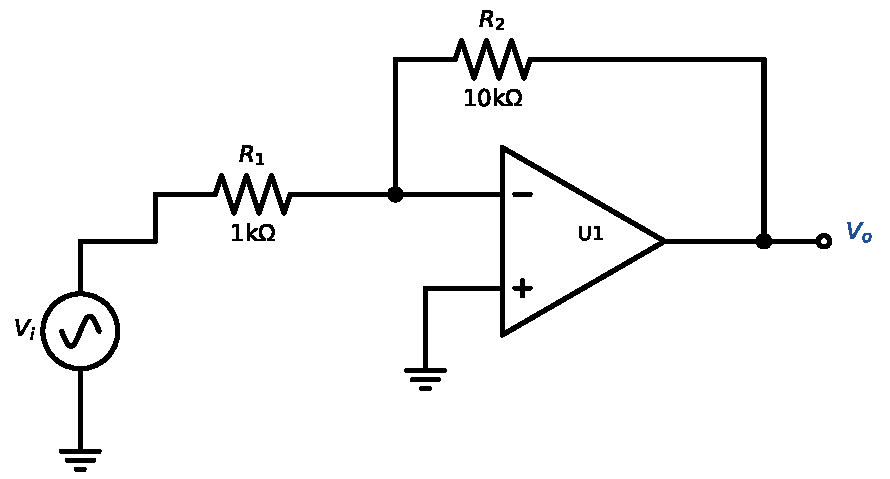
\includegraphics[width=\linewidth,height=5.6cm,keepaspectratio]{p01_circuit}\end{center}
\end{probbox}

\begin{probbox}{Problem 2E.2 \hfill Easy}
In the circuit below (ideal op-amps (except for the slew rate)), every op-amp has the slew rate $SR = 1\,\mathrm{V}/\mu\mathrm{s}$. The input is $V_i(t) = A\sin(2\pi\cdot 50000\,t)$. Find the largest amplitude $A$ for which no op-amp output is slew-rate limited.
\begin{center}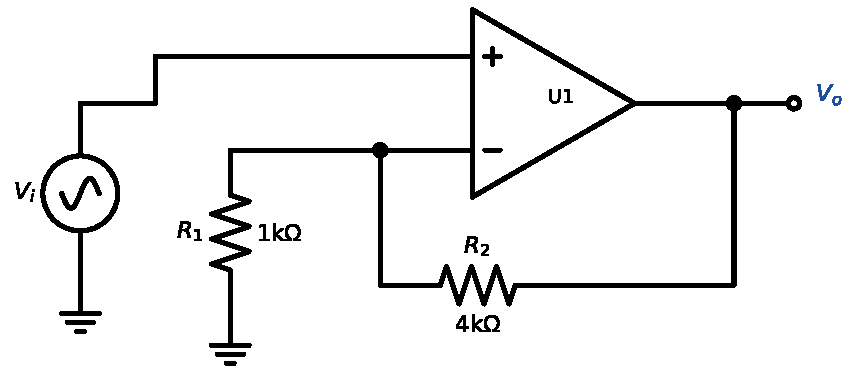
\includegraphics[width=\linewidth,height=5.6cm,keepaspectratio]{p02_circuit}\end{center}
\end{probbox}

\begin{probbox}{Problem 2E.3 \hfill Easy}
In the circuit below (ideal op-amps (except for the slew rate)), every op-amp has the slew rate $SR = 0.2\,\mathrm{V}/\mu\mathrm{s}$. The input is $V_i(t) = A\sin(2\pi\cdot 10000\,t)$. Find the largest amplitude $A$ for which no op-amp output is slew-rate limited.
\begin{center}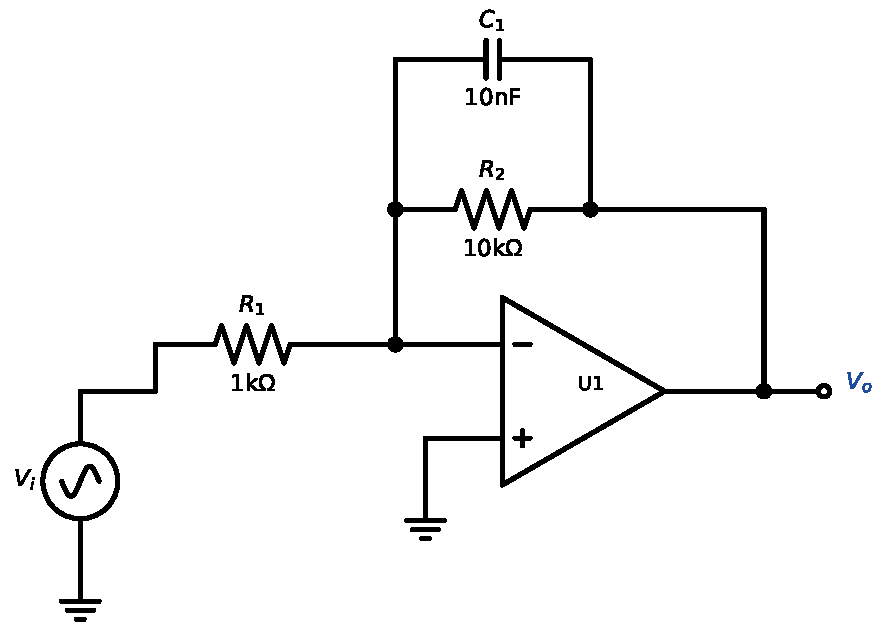
\includegraphics[width=\linewidth,height=5.6cm,keepaspectratio]{p03_circuit}\end{center}
\end{probbox}

\begin{probbox}{Problem 2E.4 \hfill Easy}
In the circuit below (ideal op-amps (except for the slew rate)), every op-amp has the slew rate $SR = 2\,\mathrm{V}/\mu\mathrm{s}$. The input is $V_i(t) = A\sin(2\pi\cdot 10000\,t)$. Find the largest amplitude $A$ for which no op-amp output is slew-rate limited.
\begin{center}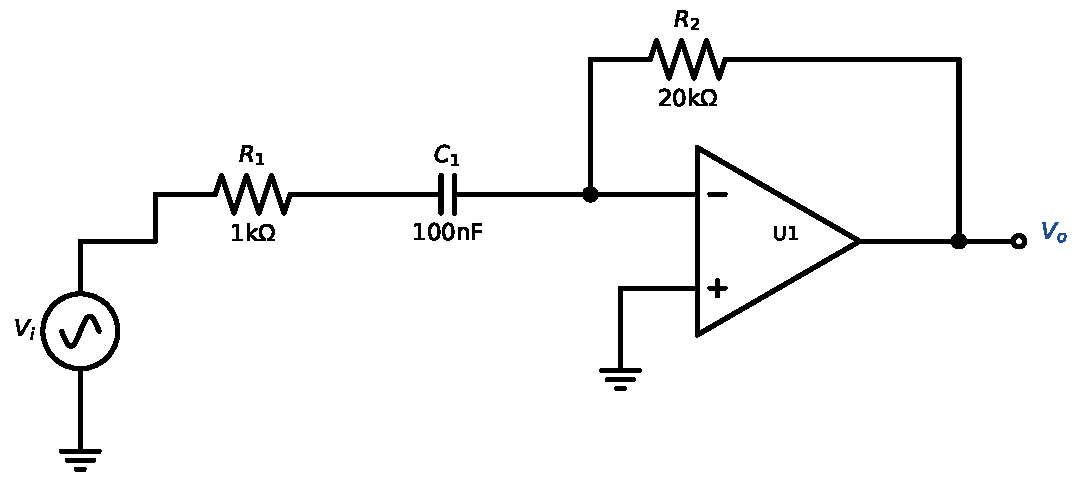
\includegraphics[width=\linewidth,height=5.6cm,keepaspectratio]{p04_circuit}\end{center}
\end{probbox}

\begin{probbox}{Problem 2E.5 \hfill Easy}
In the circuit below (ideal op-amps (except for the slew rate)), every op-amp has the slew rate $SR = 0.3\,\mathrm{V}/\mu\mathrm{s}$. The input is $V_i(t) = A\sin(2\pi\cdot 10^{5}\,t)$. Find the largest amplitude $A$ for which no op-amp output is slew-rate limited.
\begin{center}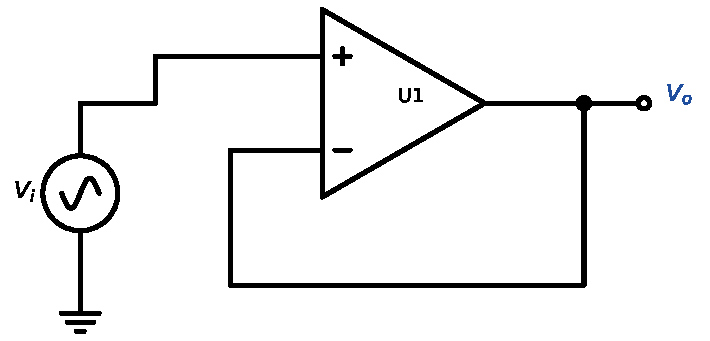
\includegraphics[width=\linewidth,height=5.6cm,keepaspectratio]{p05_circuit}\end{center}
\end{probbox}

\begin{probbox}{Problem 2E.6 \hfill Easy}
In the circuit below (ideal op-amps (except for the slew rate)), every op-amp has the slew rate $SR = 1\,\mathrm{V}/\mu\mathrm{s}$. The input is $V_i(t) = A\sin(2\pi\cdot 20000\,t)$. Find the largest amplitude $A$ for which no op-amp output is slew-rate limited.
\begin{center}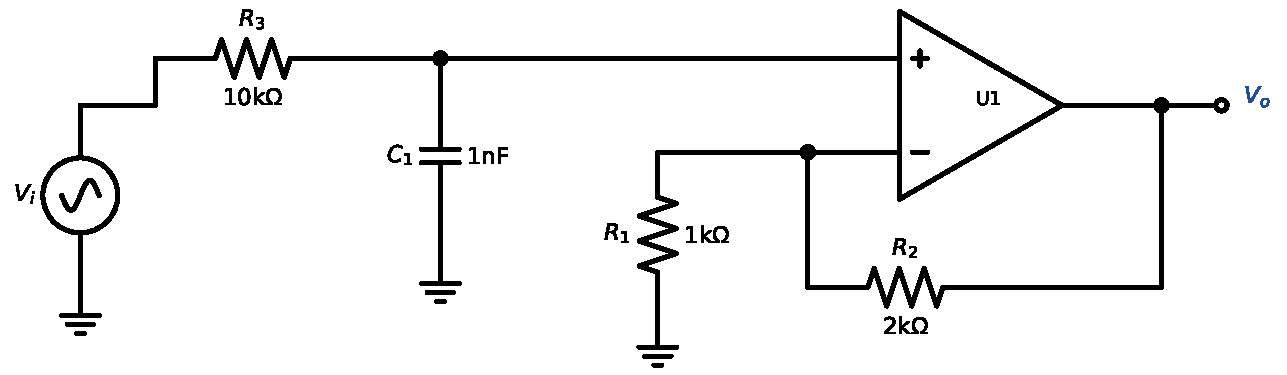
\includegraphics[width=\linewidth,height=5.6cm,keepaspectratio]{p06_circuit}\end{center}
\end{probbox}

\subsection*{Medium problems}
\begin{probbox}{Problem 2E.7 \hfill Medium}
In the circuit below (ideal op-amps (except for the slew rate)), every op-amp has the slew rate $SR = 1\,\mathrm{V}/\mu\mathrm{s}$. The input is $V_i(t) = A\sin(2\pi\cdot 50000\,t)$. Find the largest amplitude $A$ for which no op-amp output is slew-rate limited, and say which op-amp output distorts first.
\begin{center}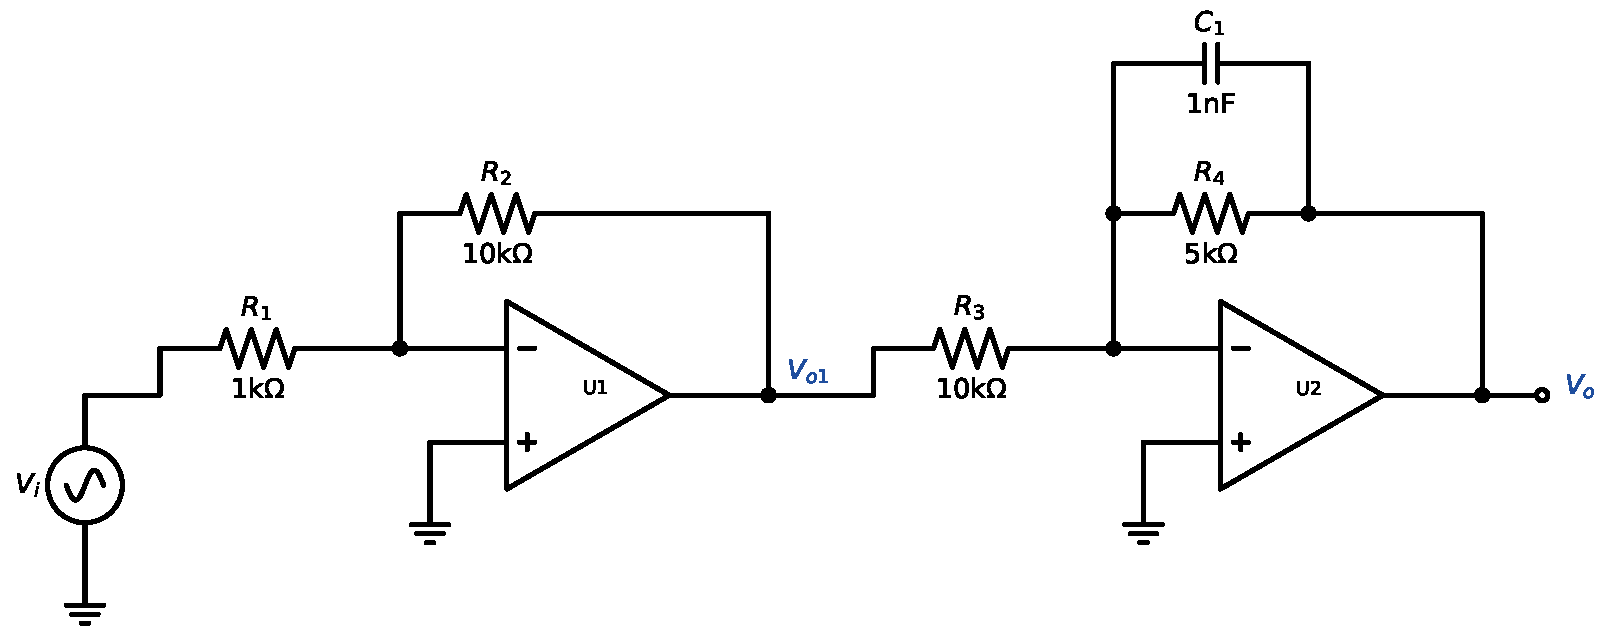
\includegraphics[width=\linewidth,height=5.6cm,keepaspectratio]{p07_circuit}\end{center}
\end{probbox}

\begin{probbox}{Problem 2E.8 \hfill Medium}
In the circuit below (ideal op-amps (except for the slew rate)), every op-amp has the slew rate $SR = 0.5\,\mathrm{V}/\mu\mathrm{s}$. The input is $V_i(t) = A\sin(2\pi\cdot 3000\,t)$. Find the largest amplitude $A$ for which no op-amp output is slew-rate limited, and say which op-amp output distorts first.
\begin{center}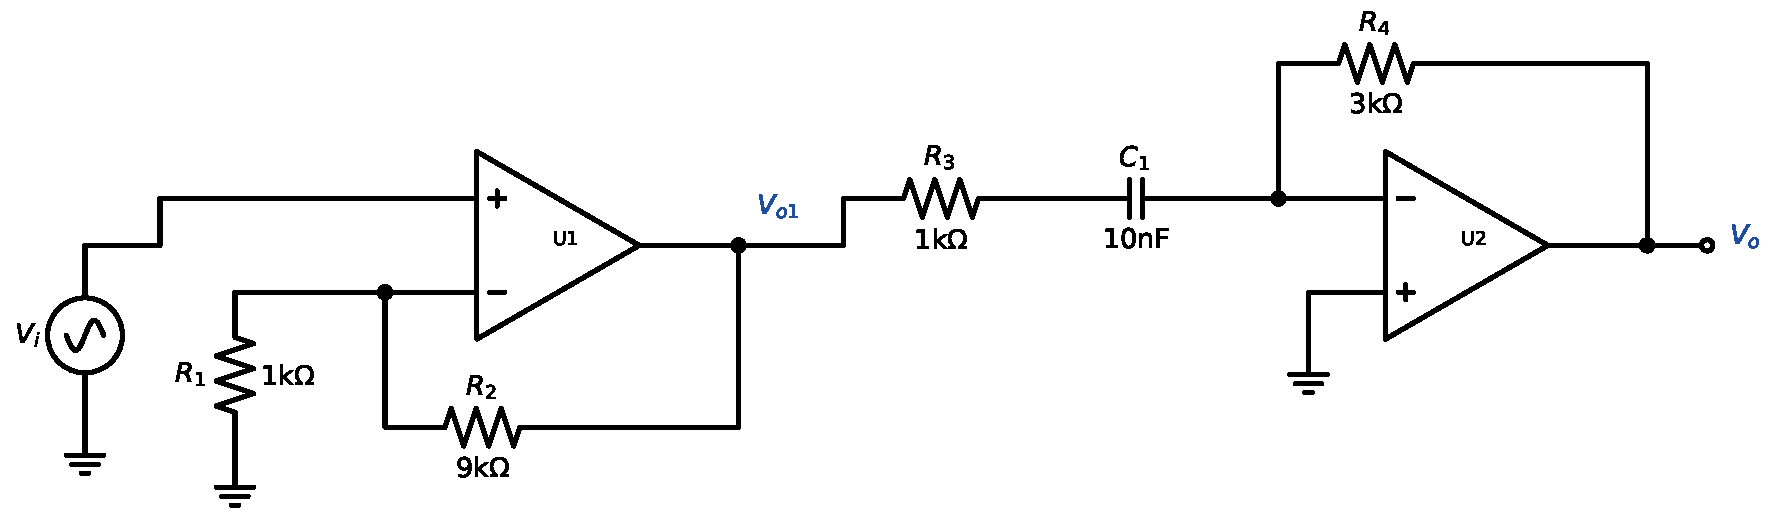
\includegraphics[width=\linewidth,height=5.6cm,keepaspectratio]{p08_circuit}\end{center}
\end{probbox}

\begin{probbox}{Problem 2E.9 \hfill Medium}
In the circuit below (ideal op-amps (except for the slew rate)), every op-amp has the slew rate $SR = 1\,\mathrm{V}/\mu\mathrm{s}$. The input is $V_i(t) = A\sin(2\pi\cdot 10000\,t)$. Find the largest amplitude $A$ for which no op-amp output is slew-rate limited, and say which op-amp output distorts first.
\begin{center}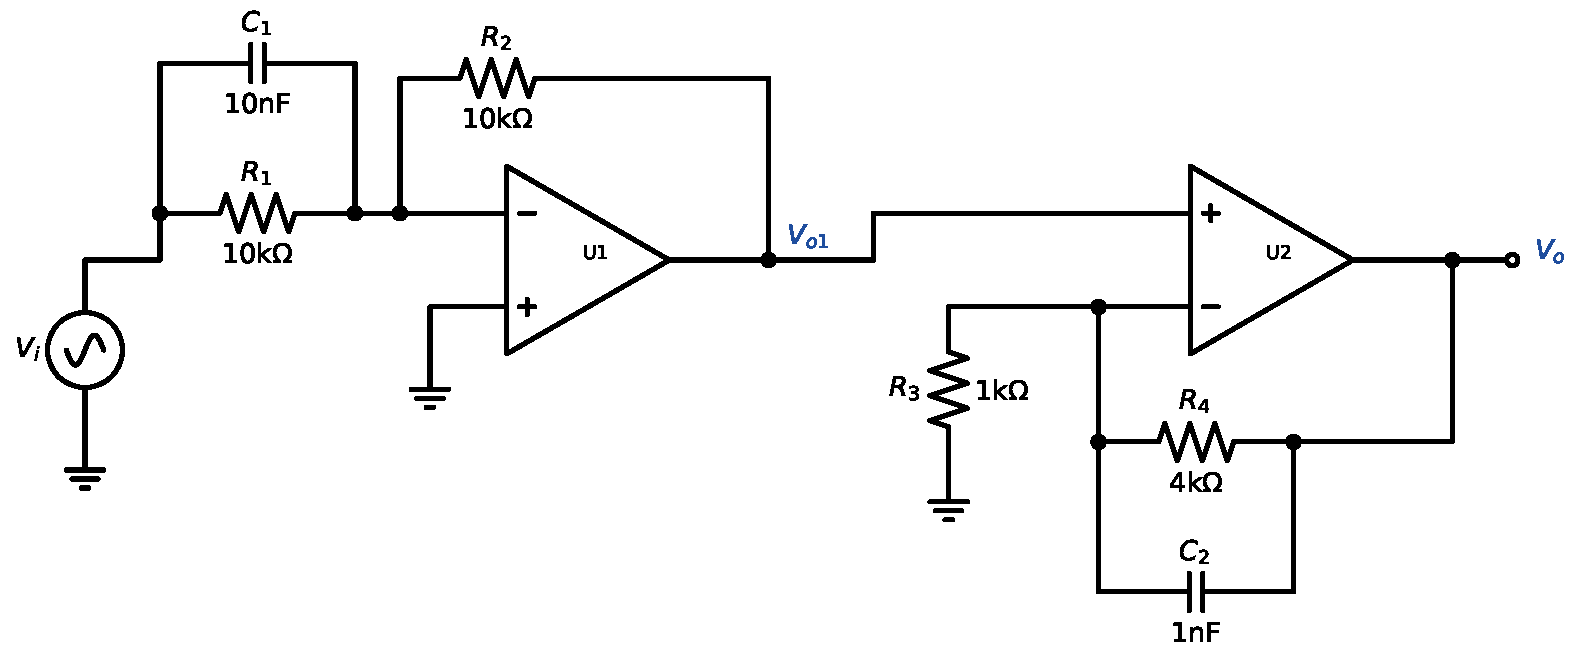
\includegraphics[width=\linewidth,height=5.6cm,keepaspectratio]{p09_circuit}\end{center}
\end{probbox}

\begin{probbox}{Problem 2E.10 \hfill Medium}
In the circuit below (op-amps with open-loop gain $A(s)=\dfrac{10^{5}}{1+\dfrac{s}{2\pi\cdot 20}}$), every op-amp has the slew rate $SR = 2\,\mathrm{V}/\mu\mathrm{s}$. The input is $V_i(t) = A\sin(2\pi\cdot 2\times 10^{5}\,t)$. Find the largest amplitude $A$ for which no op-amp output is slew-rate limited, and say which op-amp output distorts first.
\begin{center}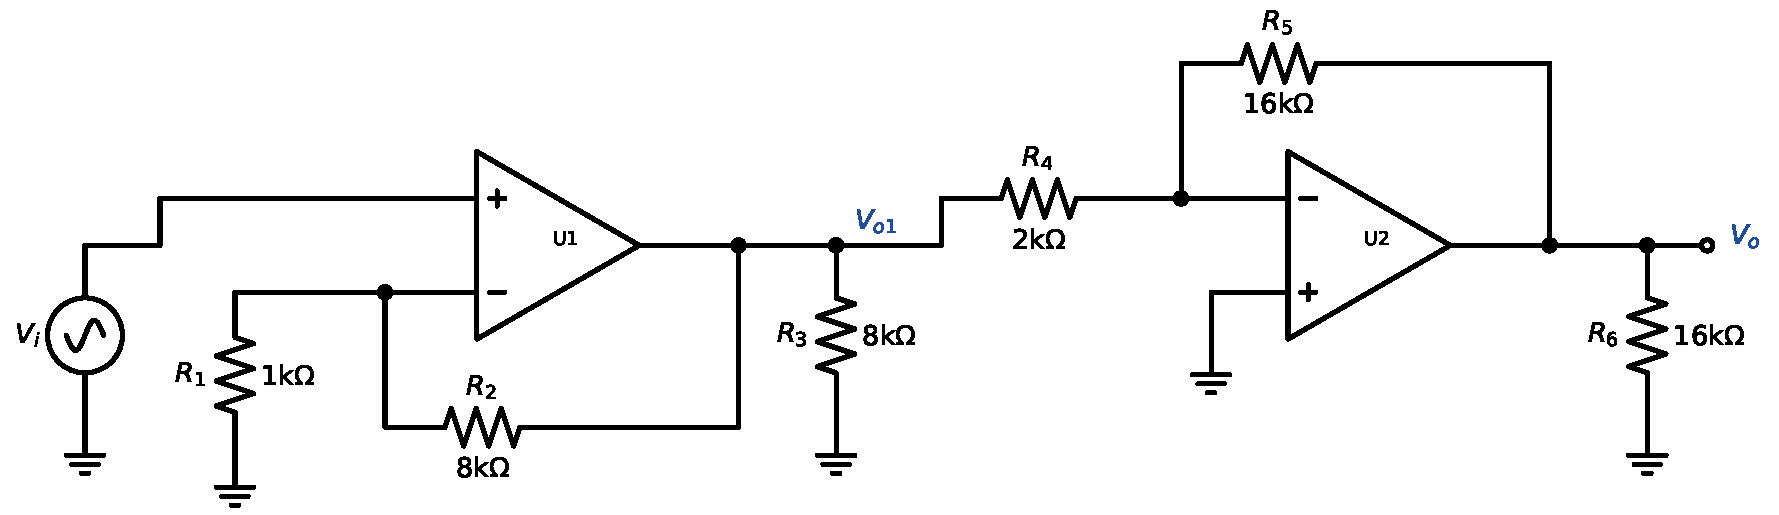
\includegraphics[width=\linewidth,height=5.6cm,keepaspectratio]{p10_circuit}\end{center}
\end{probbox}

\begin{probbox}{Problem 2E.11 \hfill Medium}
In the circuit below (op-amps with open-loop gain $A(s)=\dfrac{10^{5}}{1+\dfrac{s}{2\pi\cdot 10}}$), every op-amp has the slew rate $SR = 3\,\mathrm{V}/\mu\mathrm{s}$. The input is $V_i(t) = A\sin(2\pi\cdot 50000\,t)$. Find the largest amplitude $A$ for which no op-amp output is slew-rate limited.
\begin{center}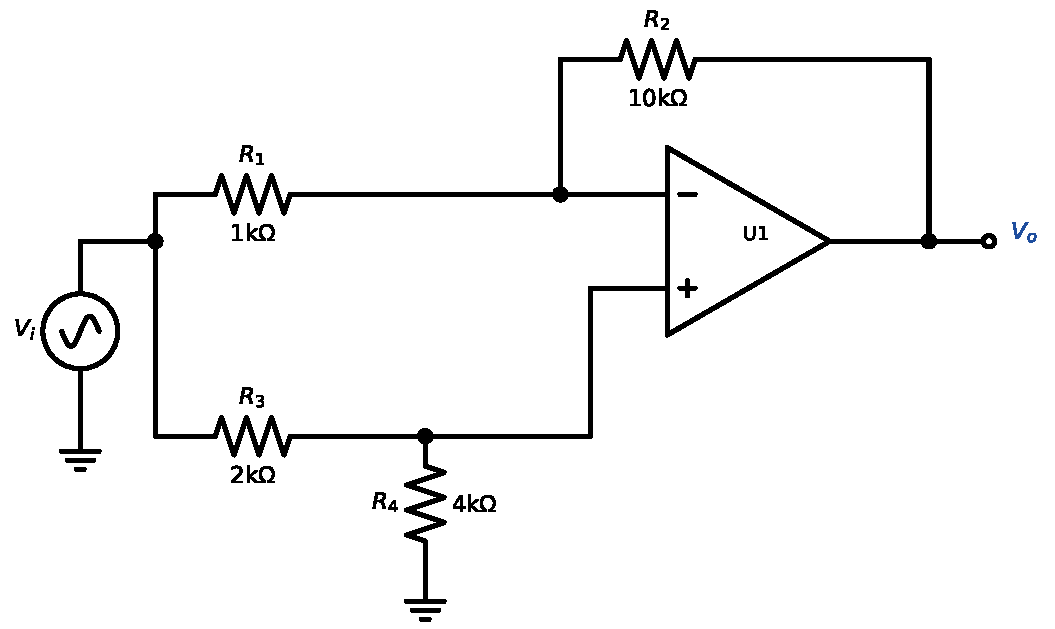
\includegraphics[width=\linewidth,height=5.6cm,keepaspectratio]{p11_circuit}\end{center}
\end{probbox}

\begin{probbox}{Problem 2E.12 \hfill Medium}
In the circuit below (ideal op-amps (except for the slew rate)), every op-amp has the slew rate $SR = 0.5\,\mathrm{V}/\mu\mathrm{s}$. The input is $V_i(t) = A\sin(2\pi\cdot 8000\,t)$. Find the largest amplitude $A$ for which no op-amp output is slew-rate limited, and say which op-amp output distorts first.
\begin{center}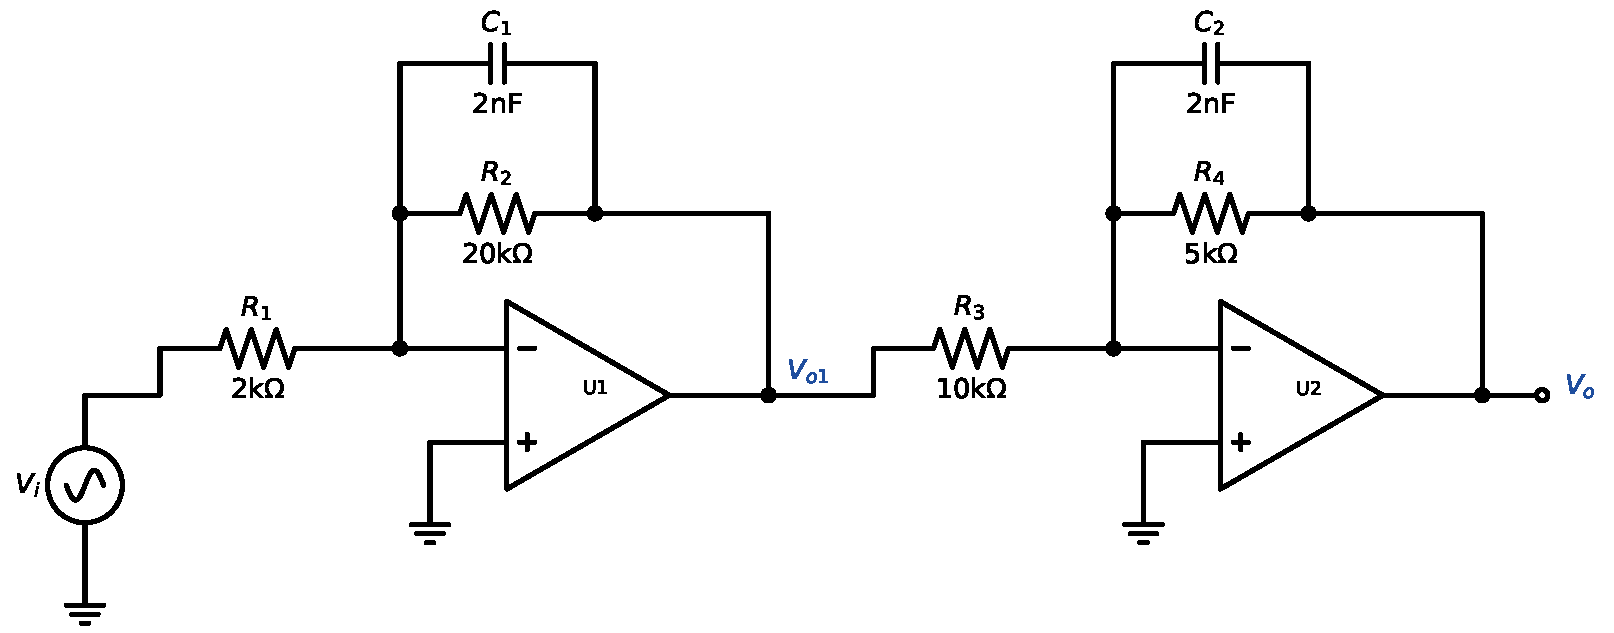
\includegraphics[width=\linewidth,height=5.6cm,keepaspectratio]{p12_circuit}\end{center}
\end{probbox}

\subsection*{Hard problems}
\begin{probbox}{Problem 2E.13 \hfill Hard}
In the circuit below (ideal op-amps (except for the slew rate)), every op-amp has the slew rate $SR = 1\,\mathrm{V}/\mu\mathrm{s}$. The input is $V_i(t) = A\sin(2\pi\cdot 20000\,t)$. Find the largest amplitude $A$ for which no op-amp output is slew-rate limited, and say which op-amp output distorts first.
\begin{center}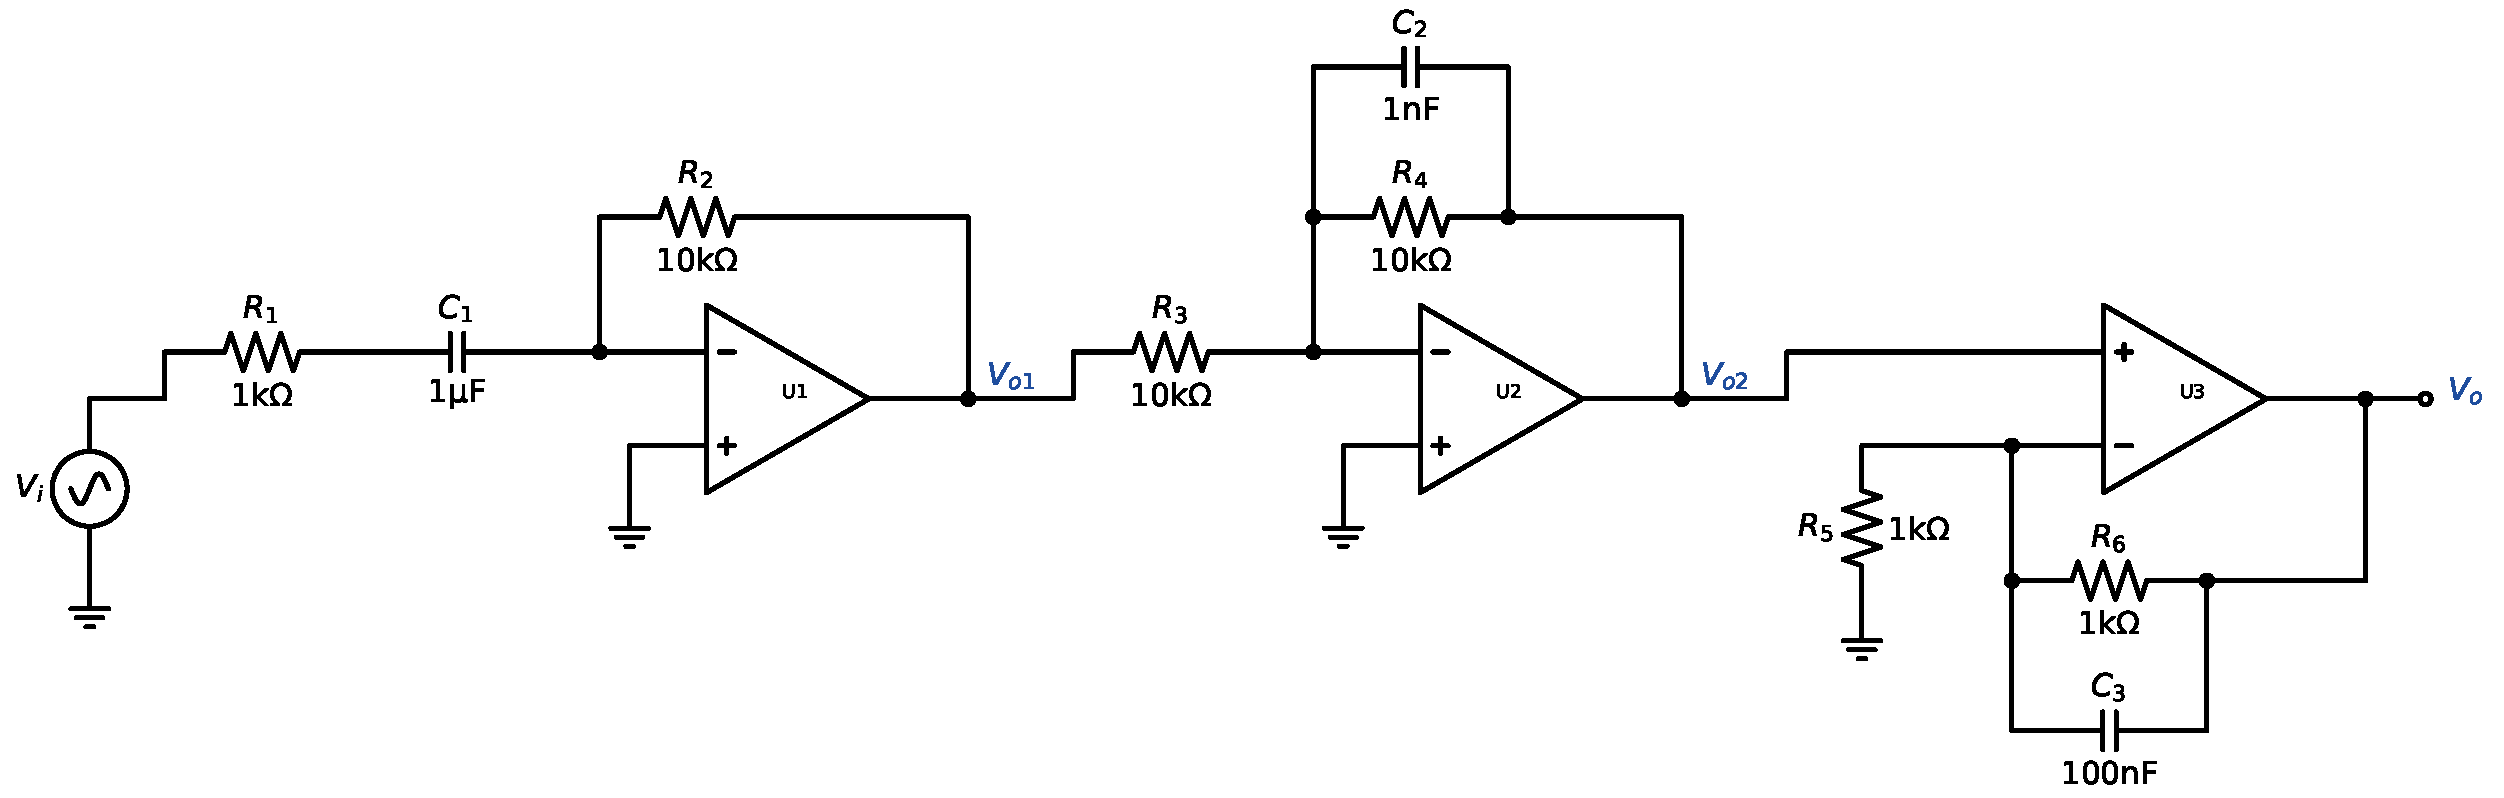
\includegraphics[width=\linewidth,height=5.6cm,keepaspectratio]{p13_circuit}\end{center}
\end{probbox}

\begin{probbox}{Problem 2E.14 \hfill Hard}
In the circuit below (ideal op-amps (except for the slew rate)), every op-amp has the slew rate $SR = 0.5\,\mathrm{V}/\mu\mathrm{s}$. The input is $V_i(t) = A\sin(2\pi\cdot 2000\,t)$. Find the largest amplitude $A$ for which no op-amp output is slew-rate limited, and say which op-amp output distorts first.
\begin{center}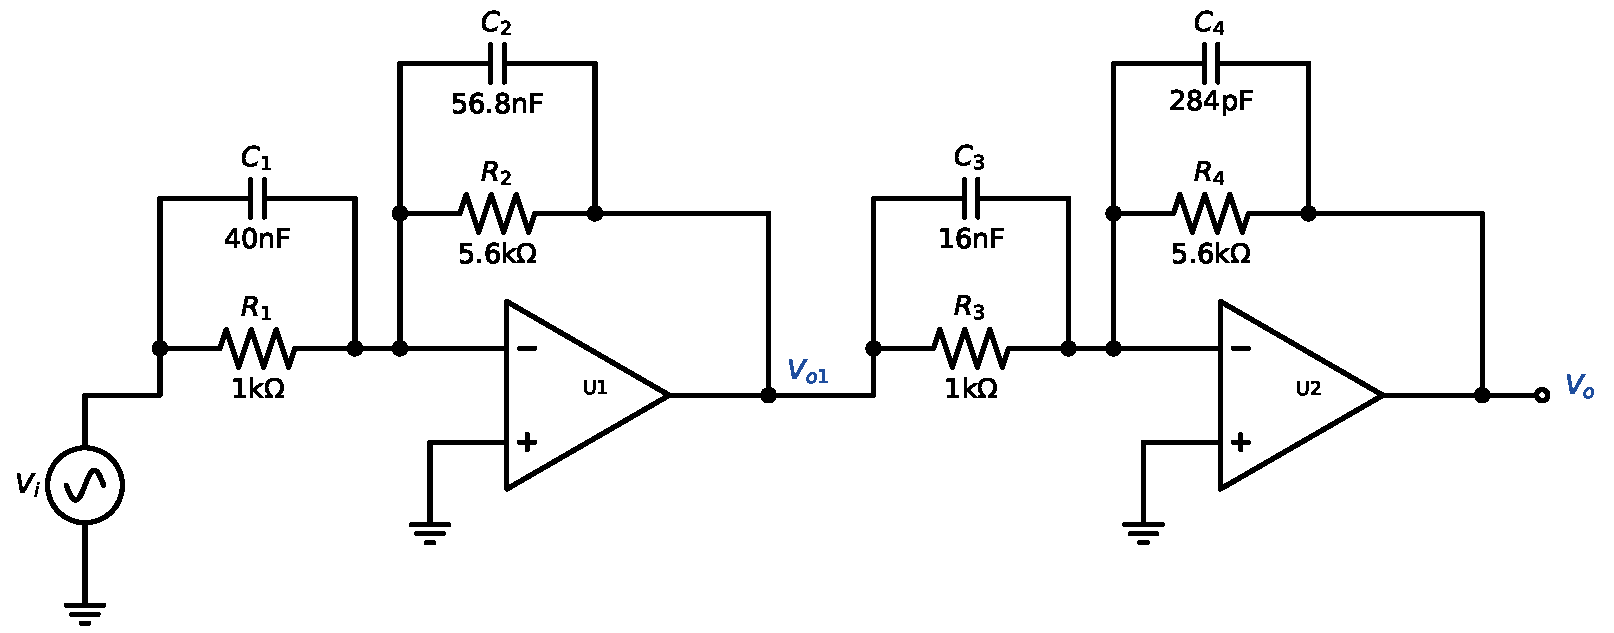
\includegraphics[width=\linewidth,height=5.6cm,keepaspectratio]{p14_circuit}\end{center}
\end{probbox}

\begin{probbox}{Problem 2E.15 \hfill Hard}
In the circuit below (op-amps with open-loop gain $A(s)=\dfrac{10^{5}}{1+\dfrac{s}{2\pi\cdot 30}}$), every op-amp has the slew rate $SR = 5\,\mathrm{V}/\mu\mathrm{s}$. The input is $V_i(t) = A\sin(2\pi\cdot 5\times 10^{5}\,t)$. Find the largest amplitude $A$ for which no op-amp output is slew-rate limited.
\begin{center}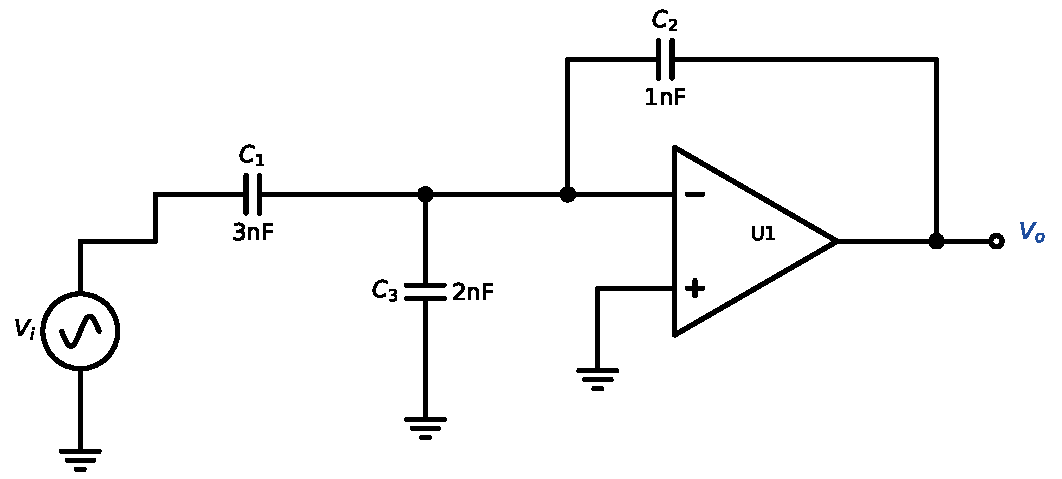
\includegraphics[width=\linewidth,height=5.6cm,keepaspectratio]{p15_circuit}\end{center}
\end{probbox}

\begin{probbox}{Problem 2E.16 \hfill Hard}
In the circuit below (op-amps with open-loop gain $A(s)=\dfrac{10^{5}}{1+\dfrac{s}{2\pi\cdot 10}}$), every op-amp has the slew rate $SR = 2\,\mathrm{V}/\mu\mathrm{s}$. The input is $V_i(t) = A\sin(2\pi\cdot 10^{5}\,t)$. Find the largest amplitude $A$ for which no op-amp output is slew-rate limited, and say which op-amp output distorts first.
\begin{center}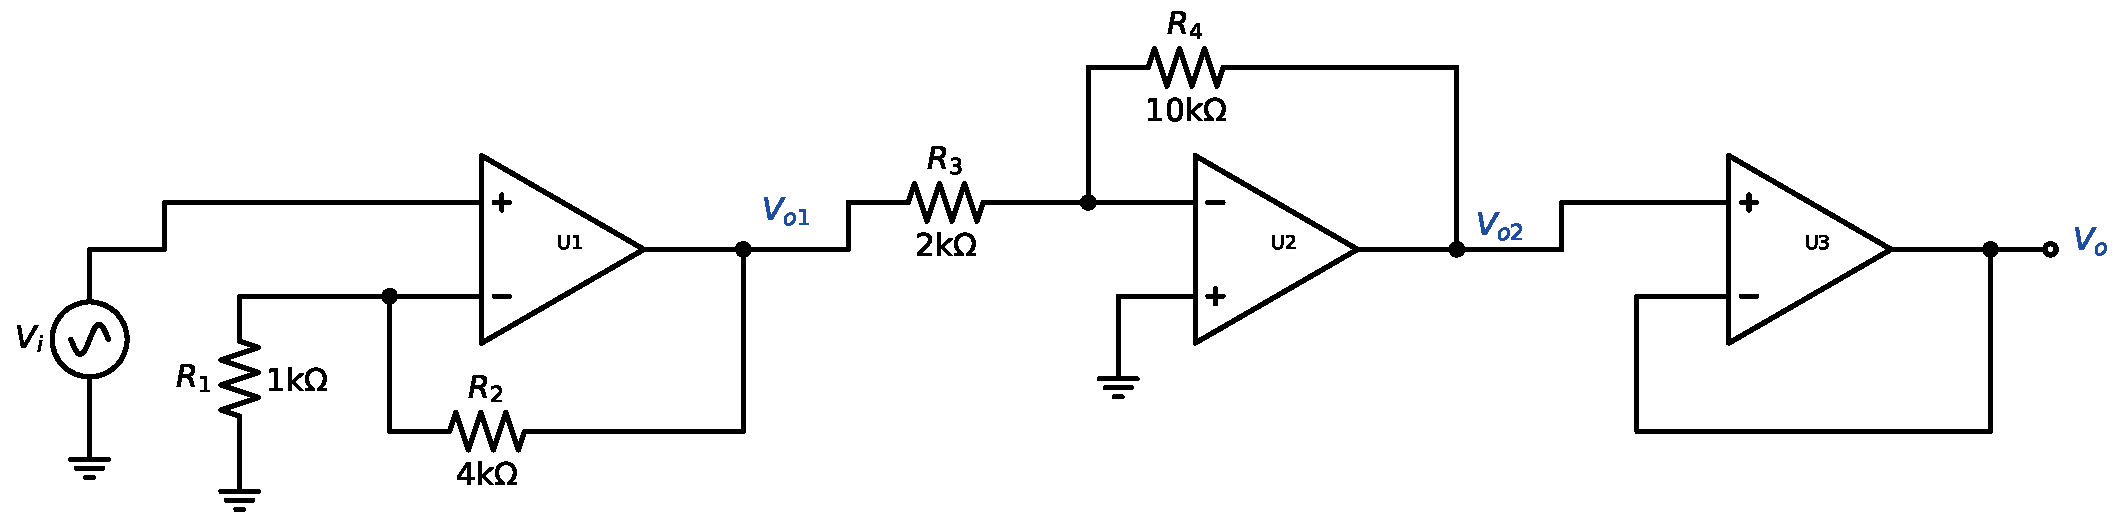
\includegraphics[width=\linewidth,height=5.6cm,keepaspectratio]{p16_circuit}\end{center}
\end{probbox}

\begin{probbox}{Problem 2E.17 \hfill Hard}
In the circuit below (ideal op-amps (except for the slew rate)), every op-amp has the slew rate $SR = 0.2\,\mathrm{V}/\mu\mathrm{s}$. The input is $V_i(t) = A\sin(2\pi\cdot 10000\,t)$. Find the largest amplitude $A$ for which no op-amp output is slew-rate limited, and say which op-amp output distorts first.
\begin{center}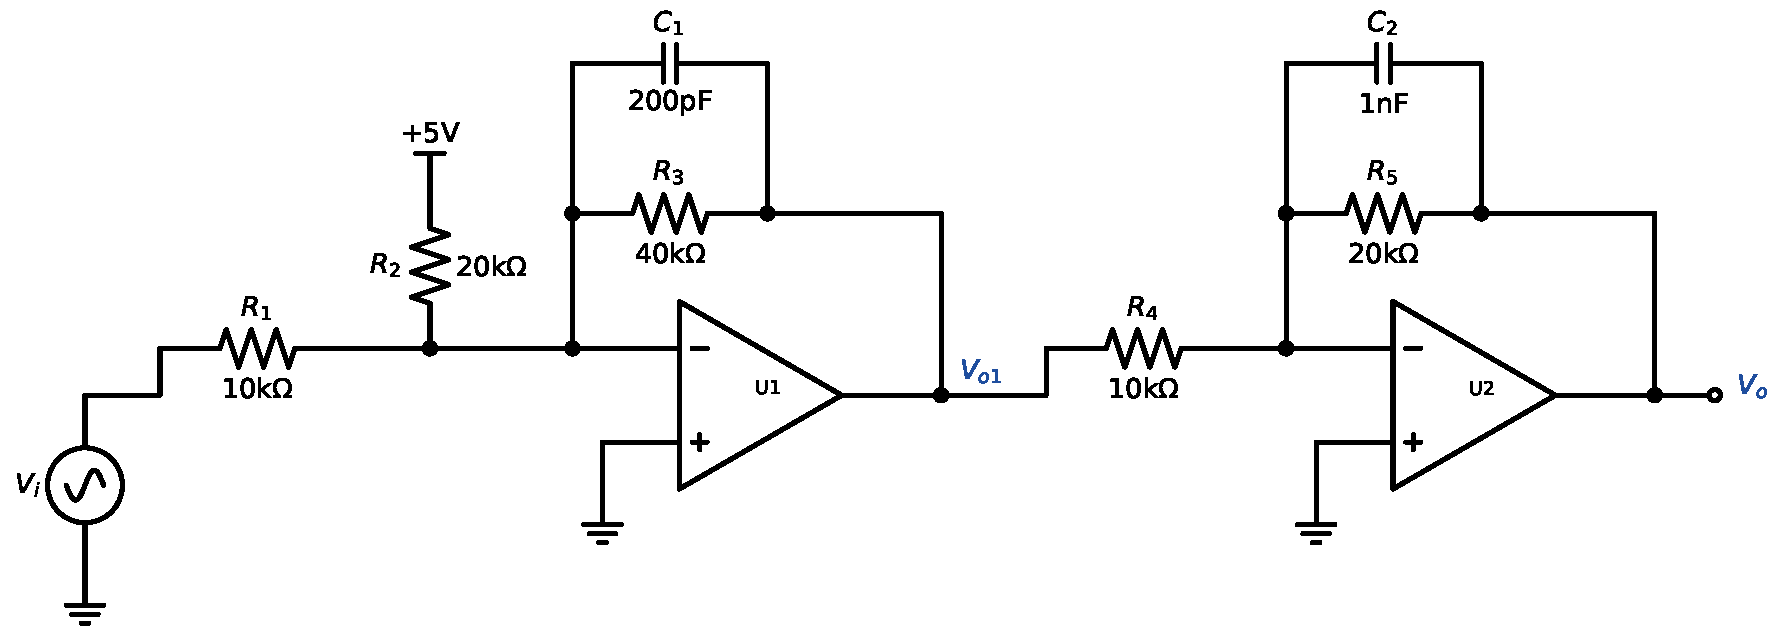
\includegraphics[width=\linewidth,height=5.6cm,keepaspectratio]{p17_circuit}\end{center}
\end{probbox}

\begin{probbox}{Problem 2E.18 \hfill Hard}
In the circuit below (ideal op-amps (except for the slew rate)), every op-amp has the slew rate $SR = 0.8\,\mathrm{V}/\mu\mathrm{s}$. The input is $V_i(t) = A\sin(2\pi\cdot 6000\,t)$. Find the largest amplitude $A$ for which no op-amp output is slew-rate limited, and say which op-amp output distorts first.
\begin{center}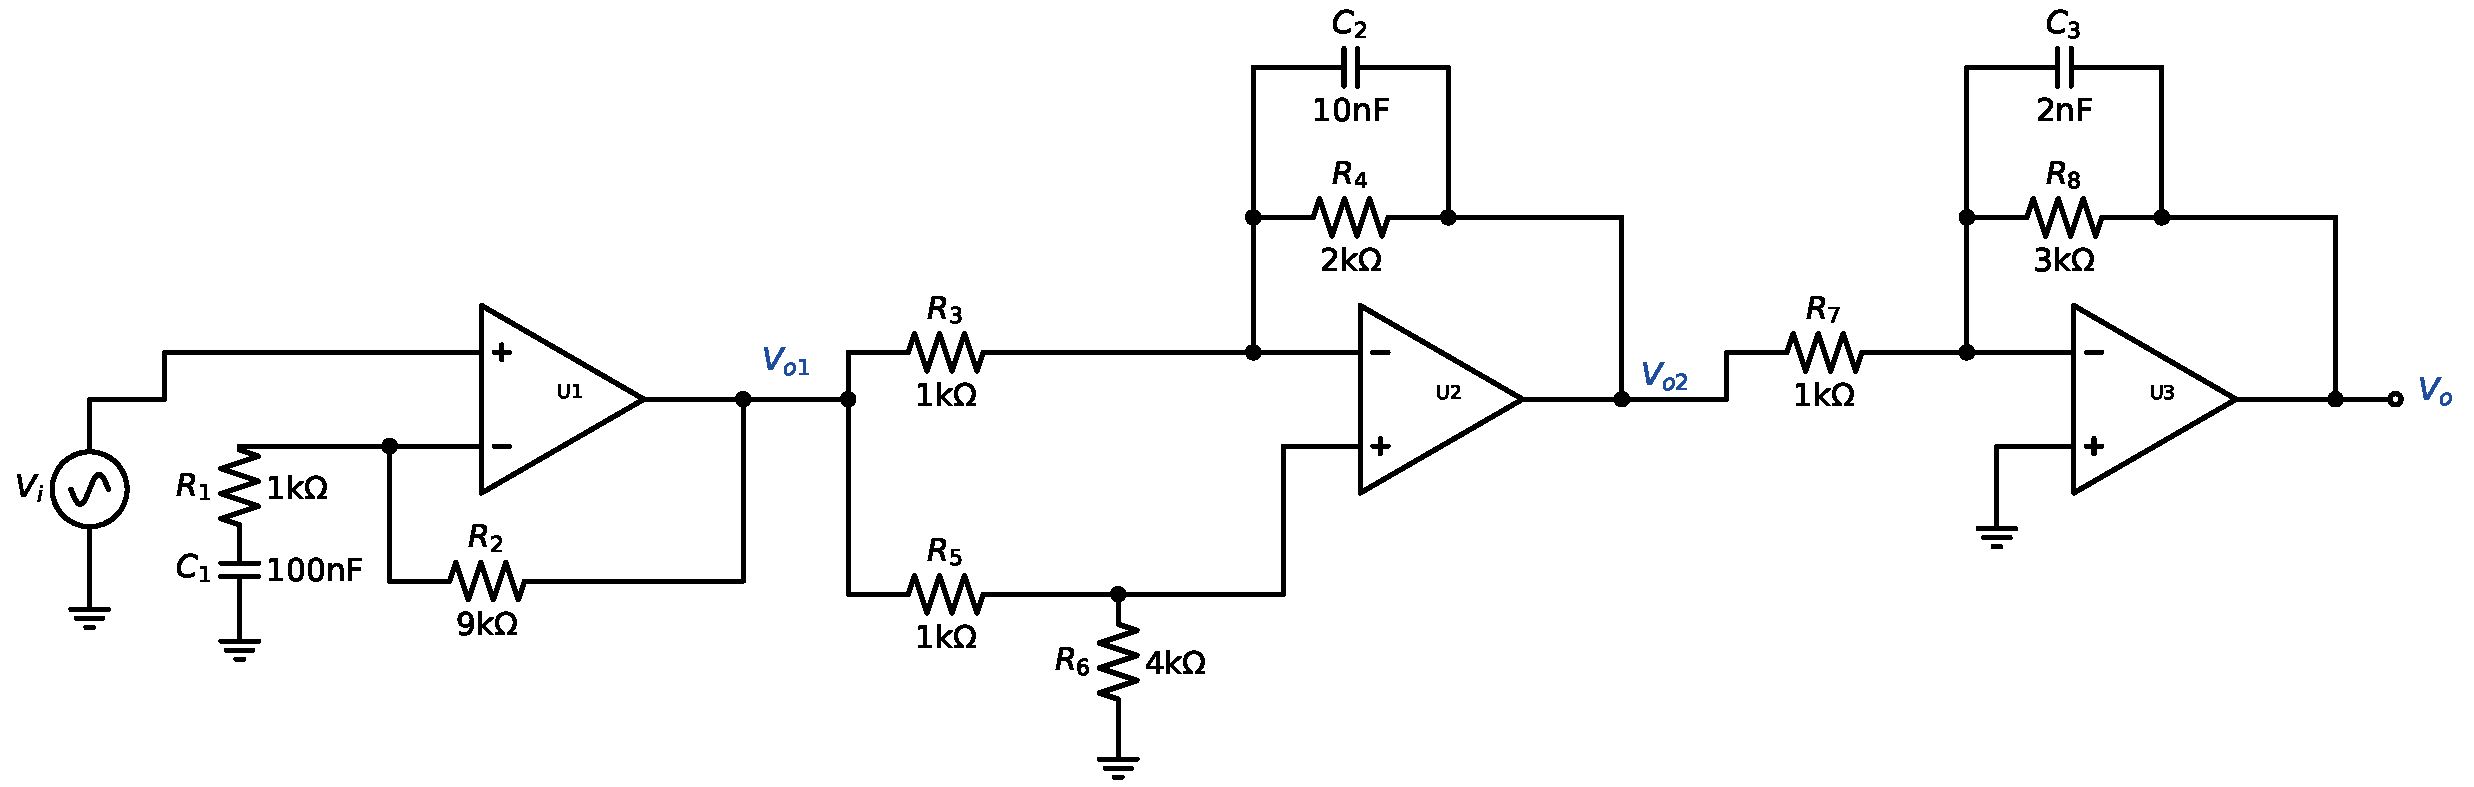
\includegraphics[width=\linewidth,height=5.6cm,keepaspectratio]{p18_circuit}\end{center}
\end{probbox}

\newpage
\section*{Solutions}
Every solution follows the steps of the Lecture-2 pipeline card.
\newpage
\subsection*{Solution 2E.1 \hfill Easy}
\begin{center}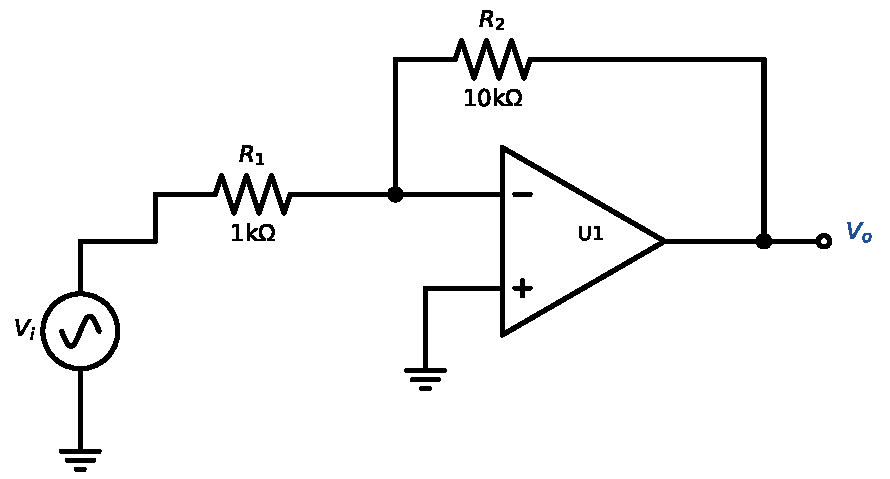
\includegraphics[width=\linewidth,height=5cm,keepaspectratio]{p01_circuit}\end{center}
\solstep{1}{What limits the input?}Every op-amp output must obey tool T6. For $V_i = A\sin(\omega_{in} t)$ each op-amp output is a sinusoid $|H_k(j\omega_{in})|A\sin(\omega_{in}t+\dots)$, so its fastest slope is $\omega_{in}|H_k(j\omega_{in})|A$. We need $|H_k(j\omega_{in})|$ from $V_i$ to the output. Here $\omega_{in} = 2\pi\cdot20000 = 1.26\times 10^{5}$\,rad/s and $SR = 0.5\,\mathrm{V}/\mu\mathrm{s} = 5\times 10^{5}\,\mathrm{V/s}$.
\solstep{2}{Gain to every op-amp output at $\omega_{in}$}Ideal op-amps: each block follows from its block formula (tool T2); a cascade multiplies, so $|H_k| = \prod_{j\le k}|\text{block } j|$.

\textbf{Block 1 (U1).} Inverting block: the $+$ input is grounded, so $V_- = V_+ = 0$ (virtual ground). The current $\frac{V_{i} - 0}{R_{1}}$ through $R_{1}$ cannot enter the op-amp, so all of it flows through $R_{2}$: $V_{o} = 0 - R_{2}\cdot\frac{V_{i}}{R_{1}}$.\[
\frac{V_{o}}{V_{i}} = -\frac{R_{2}}{R_{1}} = -10
\]
At $s=j\omega_{in}$: $\left|\frac{V_{o}}{V_{i}}\right| = 10$.

{\small (To evaluate a magnitude, put $s=j\omega_{in}$ and use $|a+jb|=\sqrt{a^2+b^2}$ for the numerator and the denominator separately.)}
\solstep{3}{Which output slews first?}\begin{center}\renewcommand{\arraystretch}{1.35}
\begin{tabular}{cccc}
\toprule
output & $|H_k(j\omega_{in})|$ & amplitude & max slope $\omega_{in}|H_k|A$ (V/s) \\
\midrule
$V_{o}$ & $10$ & $10A$ & $1.257\times 10^{6}A$ \\
\bottomrule
\end{tabular}\end{center}
There is only one op-amp output.
\solstep{4}{Maximum input amplitude}\[
\omega_{in}\,|H|\,A \le SR\ \Rightarrow\ A_{max} = \frac{SR}{\omega_{in}|H|} = \frac{5\times 10^{5}}{1.26\times 10^{5}\times10} = 398\,\mathrm{m}\mathrm{V}
\]

\begin{ansbox}
$A_{max} = 398\,\mathrm{m}\mathrm{V}$ (input amplitude); at that point $V_{o}$ has amplitude $3.98\,\mathrm{V}$.
\end{ansbox}

\newpage
\subsection*{Solution 2E.2 \hfill Easy}
\begin{center}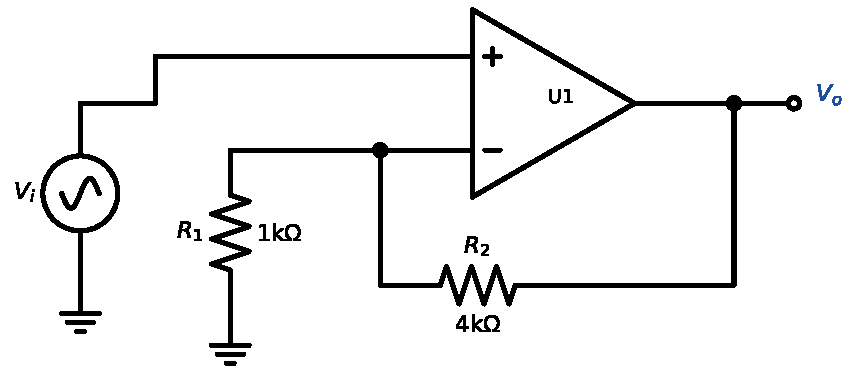
\includegraphics[width=\linewidth,height=5cm,keepaspectratio]{p02_circuit}\end{center}
\solstep{1}{What limits the input?}Every op-amp output must obey tool T6. For $V_i = A\sin(\omega_{in} t)$ each op-amp output is a sinusoid $|H_k(j\omega_{in})|A\sin(\omega_{in}t+\dots)$, so its fastest slope is $\omega_{in}|H_k(j\omega_{in})|A$. We need $|H_k(j\omega_{in})|$ from $V_i$ to the output. Here $\omega_{in} = 2\pi\cdot50000 = 3.14\times 10^{5}$\,rad/s and $SR = 1\,\mathrm{V}/\mu\mathrm{s} = 10^{6}\,\mathrm{V/s}$.
\solstep{2}{Gain to every op-amp output at $\omega_{in}$}Ideal op-amps: each block follows from its block formula (tool T2); a cascade multiplies, so $|H_k| = \prod_{j\le k}|\text{block } j|$.

\textbf{Block 1 (U1).} Non-inverting block: The $+$ input is the block input: $V_+ = V_{i}$. The op-amp forces $V_-=V_+$, and $R_{1}$, $R_{2}$ divide the output: $V_- = \frac{R_{1}}{R_{1} + R_{2}}V_{o}$, hence $V_{o} = \left(1+\frac{R_{2}}{R_{1}}\right)V_+$.\[
\frac{V_{o}}{V_{i}} = \left(1+\frac{R_{2}}{R_{1}}\right) = 5
\]
At $s=j\omega_{in}$: $\left|\frac{V_{o}}{V_{i}}\right| = 5$.

{\small (To evaluate a magnitude, put $s=j\omega_{in}$ and use $|a+jb|=\sqrt{a^2+b^2}$ for the numerator and the denominator separately.)}
\solstep{3}{Which output slews first?}\begin{center}\renewcommand{\arraystretch}{1.35}
\begin{tabular}{cccc}
\toprule
output & $|H_k(j\omega_{in})|$ & amplitude & max slope $\omega_{in}|H_k|A$ (V/s) \\
\midrule
$V_{o}$ & $5$ & $5A$ & $1.571\times 10^{6}A$ \\
\bottomrule
\end{tabular}\end{center}
There is only one op-amp output.
\solstep{4}{Maximum input amplitude}\[
\omega_{in}\,|H|\,A \le SR\ \Rightarrow\ A_{max} = \frac{SR}{\omega_{in}|H|} = \frac{10^{6}}{3.14\times 10^{5}\times5} = 637\,\mathrm{m}\mathrm{V}
\]

\begin{ansbox}
$A_{max} = 637\,\mathrm{m}\mathrm{V}$ (input amplitude); at that point $V_{o}$ has amplitude $3.18\,\mathrm{V}$.
\end{ansbox}

\newpage
\subsection*{Solution 2E.3 \hfill Easy}
\begin{center}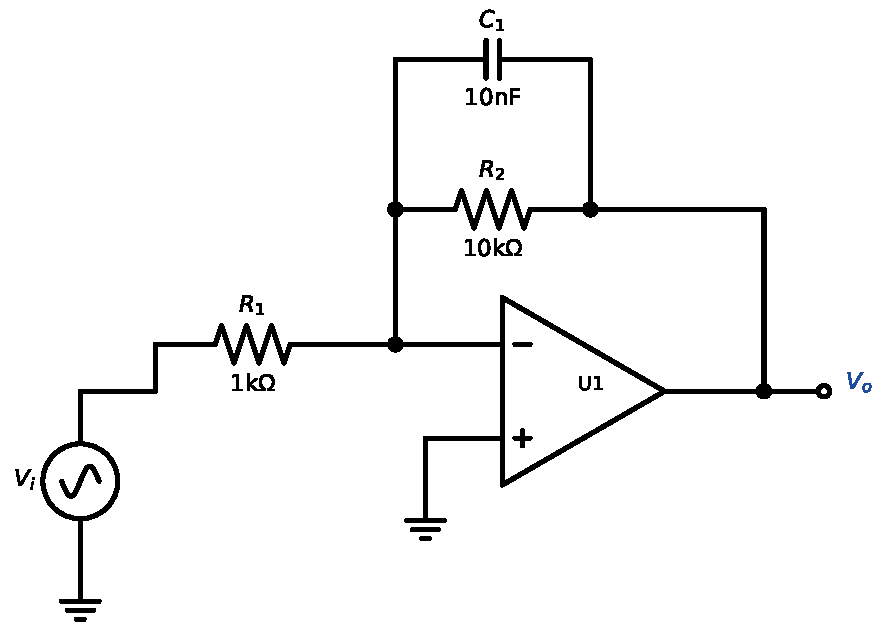
\includegraphics[width=\linewidth,height=5cm,keepaspectratio]{p03_circuit}\end{center}
\solstep{1}{What limits the input?}Every op-amp output must obey tool T6. For $V_i = A\sin(\omega_{in} t)$ each op-amp output is a sinusoid $|H_k(j\omega_{in})|A\sin(\omega_{in}t+\dots)$, so its fastest slope is $\omega_{in}|H_k(j\omega_{in})|A$. We need $|H_k(j\omega_{in})|$ from $V_i$ to the output. Here $\omega_{in} = 2\pi\cdot10000 = 62800$\,rad/s and $SR = 0.2\,\mathrm{V}/\mu\mathrm{s} = 2\times 10^{5}\,\mathrm{V/s}$.
\solstep{2}{Gain to every op-amp output at $\omega_{in}$}Ideal op-amps: each block follows from its block formula (tool T2); a cascade multiplies, so $|H_k| = \prod_{j\le k}|\text{block } j|$.

\textbf{Block 1 (U1).} Inverting block: the $+$ input is grounded, so $V_- = V_+ = 0$ (virtual ground). The current $\frac{V_{i} - 0}{R_{1}}$ through $R_{1}$ cannot enter the op-amp, so all of it flows through $Z_{f1}$: $V_{o} = 0 - Z_{f1}\cdot\frac{V_{i}}{R_{1}}$.\begin{align*}
Z_{f1} &= R_{2} \parallel \frac{1}{sC_{1}} = \dfrac{10^{8}}{s + 10000}
\end{align*}
\[
\frac{V_{o}}{V_{i}} = -\frac{Z_{f1}}{R_{1}} = \dfrac{-10^{5}}{s + 10000}
\]
At $s=j\omega_{in}$: $\left|\frac{V_{o}}{V_{i}}\right| = 1.572$.

{\small (To evaluate a magnitude, put $s=j\omega_{in}$ and use $|a+jb|=\sqrt{a^2+b^2}$ for the numerator and the denominator separately.)}
\solstep{3}{Which output slews first?}\begin{center}\renewcommand{\arraystretch}{1.35}
\begin{tabular}{cccc}
\toprule
output & $|H_k(j\omega_{in})|$ & amplitude & max slope $\omega_{in}|H_k|A$ (V/s) \\
\midrule
$V_{o}$ & $1.572$ & $1.572A$ & $98760A$ \\
\bottomrule
\end{tabular}\end{center}
There is only one op-amp output.
\solstep{4}{Maximum input amplitude}\[
\omega_{in}\,|H|\,A \le SR\ \Rightarrow\ A_{max} = \frac{SR}{\omega_{in}|H|} = \frac{2\times 10^{5}}{62800\times1.572} = 2.03\,\mathrm{V}
\]

\begin{ansbox}
$A_{max} = 2.03\,\mathrm{V}$ (input amplitude); at that point $V_{o}$ has amplitude $3.18\,\mathrm{V}$.
\end{ansbox}

\newpage
\subsection*{Solution 2E.4 \hfill Easy}
\begin{center}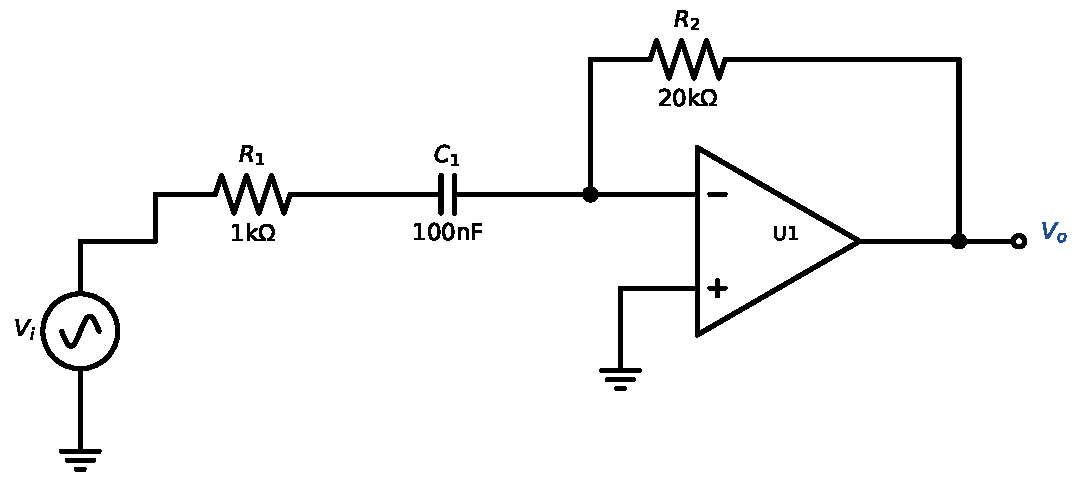
\includegraphics[width=\linewidth,height=5cm,keepaspectratio]{p04_circuit}\end{center}
\solstep{1}{What limits the input?}Every op-amp output must obey tool T6. For $V_i = A\sin(\omega_{in} t)$ each op-amp output is a sinusoid $|H_k(j\omega_{in})|A\sin(\omega_{in}t+\dots)$, so its fastest slope is $\omega_{in}|H_k(j\omega_{in})|A$. We need $|H_k(j\omega_{in})|$ from $V_i$ to the output. Here $\omega_{in} = 2\pi\cdot10000 = 62800$\,rad/s and $SR = 2\,\mathrm{V}/\mu\mathrm{s} = 2\times 10^{6}\,\mathrm{V/s}$.
\solstep{2}{Gain to every op-amp output at $\omega_{in}$}Ideal op-amps: each block follows from its block formula (tool T2); a cascade multiplies, so $|H_k| = \prod_{j\le k}|\text{block } j|$.

\textbf{Block 1 (U1).} Inverting block: the $+$ input is grounded, so $V_- = V_+ = 0$ (virtual ground). The current $\frac{V_{i} - 0}{Z_{in1}}$ through $Z_{in1}$ cannot enter the op-amp, so all of it flows through $R_{2}$: $V_{o} = 0 - R_{2}\cdot\frac{V_{i}}{Z_{in1}}$.\begin{align*}
Z_{in1} &= R_{1} + \frac{1}{sC_{1}} = \dfrac{1000\,s + 10^{7}}{s}
\end{align*}
\[
\frac{V_{o}}{V_{i}} = -\frac{R_{2}}{Z_{in1}} = \dfrac{-20\,s}{s + 10000}
\]
At $s=j\omega_{in}$: $\left|\frac{V_{o}}{V_{i}}\right| = 19.75$.

{\small (To evaluate a magnitude, put $s=j\omega_{in}$ and use $|a+jb|=\sqrt{a^2+b^2}$ for the numerator and the denominator separately.)}
\solstep{3}{Which output slews first?}\begin{center}\renewcommand{\arraystretch}{1.35}
\begin{tabular}{cccc}
\toprule
output & $|H_k(j\omega_{in})|$ & amplitude & max slope $\omega_{in}|H_k|A$ (V/s) \\
\midrule
$V_{o}$ & $19.75$ & $19.75A$ & $1.241\times 10^{6}A$ \\
\bottomrule
\end{tabular}\end{center}
There is only one op-amp output.
\solstep{4}{Maximum input amplitude}\[
\omega_{in}\,|H|\,A \le SR\ \Rightarrow\ A_{max} = \frac{SR}{\omega_{in}|H|} = \frac{2\times 10^{6}}{62800\times19.75} = 1.61\,\mathrm{V}
\]

\begin{ansbox}
$A_{max} = 1.61\,\mathrm{V}$ (input amplitude); at that point $V_{o}$ has amplitude $31.8\,\mathrm{V}$.
\end{ansbox}

\newpage
\subsection*{Solution 2E.5 \hfill Easy}
\begin{center}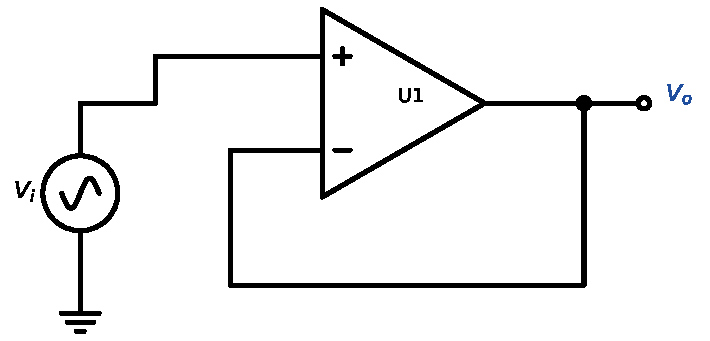
\includegraphics[width=\linewidth,height=5cm,keepaspectratio]{p05_circuit}\end{center}
\solstep{1}{What limits the input?}Every op-amp output must obey tool T6. For $V_i = A\sin(\omega_{in} t)$ each op-amp output is a sinusoid $|H_k(j\omega_{in})|A\sin(\omega_{in}t+\dots)$, so its fastest slope is $\omega_{in}|H_k(j\omega_{in})|A$. We need $|H_k(j\omega_{in})|$ from $V_i$ to the output. Here $\omega_{in} = 2\pi\cdot10^{5} = 6.28\times 10^{5}$\,rad/s and $SR = 0.3\,\mathrm{V}/\mu\mathrm{s} = 3\times 10^{5}\,\mathrm{V/s}$.
\solstep{2}{Gain to every op-amp output at $\omega_{in}$}Ideal op-amps: each block follows from its block formula (tool T2); a cascade multiplies, so $|H_k| = \prod_{j\le k}|\text{block } j|$.

\textbf{Block 1 (U1).} Non-inverting block: The $+$ input is the block input: $V_+ = V_{i}$. The output is tied back to the $-$ input, so $V_{o} = V_- = V_+$ (voltage follower).\[
\frac{V_{o}}{V_{i}} = 1 = 1
\]
At $s=j\omega_{in}$: $\left|\frac{V_{o}}{V_{i}}\right| = 1$.

{\small (To evaluate a magnitude, put $s=j\omega_{in}$ and use $|a+jb|=\sqrt{a^2+b^2}$ for the numerator and the denominator separately.)}
\solstep{3}{Which output slews first?}\begin{center}\renewcommand{\arraystretch}{1.35}
\begin{tabular}{cccc}
\toprule
output & $|H_k(j\omega_{in})|$ & amplitude & max slope $\omega_{in}|H_k|A$ (V/s) \\
\midrule
$V_{o}$ & $1$ & $1A$ & $6.283\times 10^{5}A$ \\
\bottomrule
\end{tabular}\end{center}
There is only one op-amp output.
\solstep{4}{Maximum input amplitude}\[
\omega_{in}\,|H|\,A \le SR\ \Rightarrow\ A_{max} = \frac{SR}{\omega_{in}|H|} = \frac{3\times 10^{5}}{6.28\times 10^{5}\times1} = 477\,\mathrm{m}\mathrm{V}
\]

\begin{ansbox}
$A_{max} = 477\,\mathrm{m}\mathrm{V}$ (input amplitude); at that point $V_{o}$ has amplitude $477\,\mathrm{m}\mathrm{V}$.
\end{ansbox}

\newpage
\subsection*{Solution 2E.6 \hfill Easy}
\begin{center}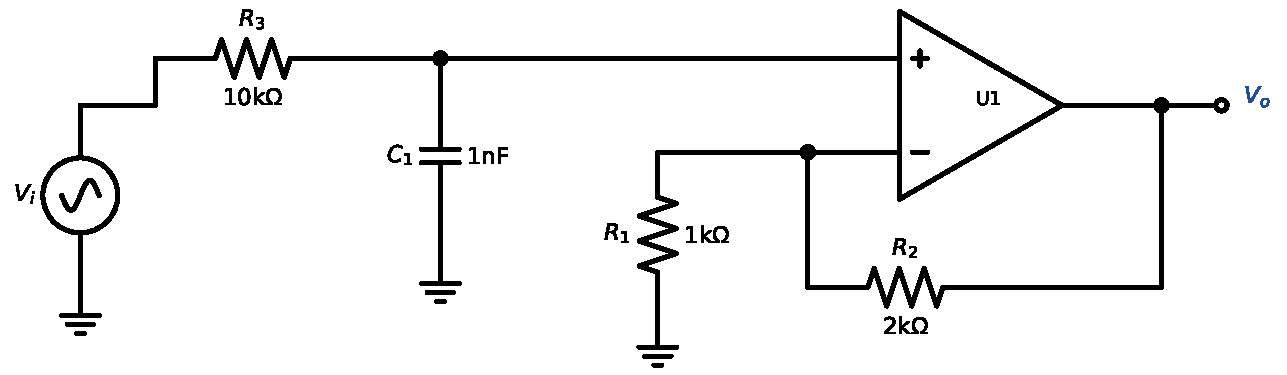
\includegraphics[width=\linewidth,height=5cm,keepaspectratio]{p06_circuit}\end{center}
\solstep{1}{What limits the input?}Every op-amp output must obey tool T6. For $V_i = A\sin(\omega_{in} t)$ each op-amp output is a sinusoid $|H_k(j\omega_{in})|A\sin(\omega_{in}t+\dots)$, so its fastest slope is $\omega_{in}|H_k(j\omega_{in})|A$. We need $|H_k(j\omega_{in})|$ from $V_i$ to the output. Here $\omega_{in} = 2\pi\cdot20000 = 1.26\times 10^{5}$\,rad/s and $SR = 1\,\mathrm{V}/\mu\mathrm{s} = 10^{6}\,\mathrm{V/s}$.
\solstep{2}{Gain to every op-amp output at $\omega_{in}$}Ideal op-amps: each block follows from its block formula (tool T2); a cascade multiplies, so $|H_k| = \prod_{j\le k}|\text{block } j|$.

\textbf{Block 1 (U1).} Non-inverting block: No current flows into the $+$ input, so $\frac{1}{sC_{1}}$ and $R_{3}$ form a plain voltage divider: $V_+ = \frac{\frac{1}{sC_{1}}}{R_{3} + \frac{1}{sC_{1}}}V_{i}$. The op-amp forces $V_-=V_+$, and $R_{1}$, $R_{2}$ divide the output: $V_- = \frac{R_{1}}{R_{1} + R_{2}}V_{o}$, hence $V_{o} = \left(1+\frac{R_{2}}{R_{1}}\right)V_+$.\[
\frac{V_{o}}{V_{i}} = \frac{\frac{1}{sC_{1}}}{R_{3} + \frac{1}{sC_{1}}}\left(1+\frac{R_{2}}{R_{1}}\right) = \dfrac{3\times 10^{5}}{s + 10^{5}}
\]
At $s=j\omega_{in}$: $\left|\frac{V_{o}}{V_{i}}\right| = 1.868$.

{\small (To evaluate a magnitude, put $s=j\omega_{in}$ and use $|a+jb|=\sqrt{a^2+b^2}$ for the numerator and the denominator separately.)}
\solstep{3}{Which output slews first?}\begin{center}\renewcommand{\arraystretch}{1.35}
\begin{tabular}{cccc}
\toprule
output & $|H_k(j\omega_{in})|$ & amplitude & max slope $\omega_{in}|H_k|A$ (V/s) \\
\midrule
$V_{o}$ & $1.868$ & $1.868A$ & $2.347\times 10^{5}A$ \\
\bottomrule
\end{tabular}\end{center}
There is only one op-amp output.
\solstep{4}{Maximum input amplitude}\[
\omega_{in}\,|H|\,A \le SR\ \Rightarrow\ A_{max} = \frac{SR}{\omega_{in}|H|} = \frac{10^{6}}{1.26\times 10^{5}\times1.868} = 4.26\,\mathrm{V}
\]

\begin{ansbox}
$A_{max} = 4.26\,\mathrm{V}$ (input amplitude); at that point $V_{o}$ has amplitude $7.96\,\mathrm{V}$.
\end{ansbox}

\newpage
\subsection*{Solution 2E.7 \hfill Medium}
\begin{center}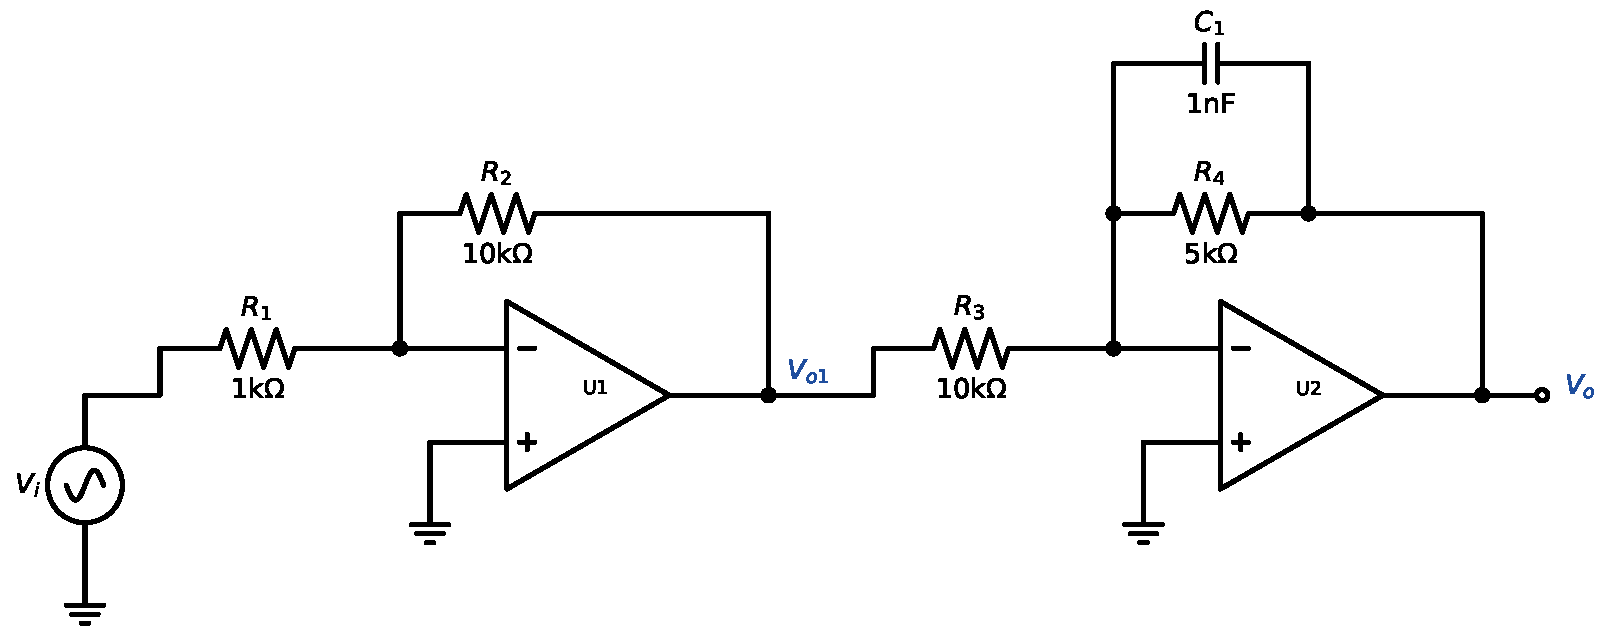
\includegraphics[width=\linewidth,height=5cm,keepaspectratio]{p07_circuit}\end{center}
\solstep{1}{What limits the input?}Every op-amp output must obey tool T6. For $V_i = A\sin(\omega_{in} t)$ each op-amp output is a sinusoid $|H_k(j\omega_{in})|A\sin(\omega_{in}t+\dots)$, so its fastest slope is $\omega_{in}|H_k(j\omega_{in})|A$. We need $|H_k(j\omega_{in})|$ from $V_i$ to each op-amp output ($V_{o1}$, $V_{o}$). Here $\omega_{in} = 2\pi\cdot50000 = 3.14\times 10^{5}$\,rad/s and $SR = 1\,\mathrm{V}/\mu\mathrm{s} = 10^{6}\,\mathrm{V/s}$.
\solstep{2}{Gain to every op-amp output at $\omega_{in}$}Ideal op-amps: each block follows from its block formula (tool T2); a cascade multiplies, so $|H_k| = \prod_{j\le k}|\text{block } j|$.

\textbf{Block 1 (U1).} Inverting block: the $+$ input is grounded, so $V_- = V_+ = 0$ (virtual ground). The current $\frac{V_{i} - 0}{R_{1}}$ through $R_{1}$ cannot enter the op-amp, so all of it flows through $R_{2}$: $V_{o1} = 0 - R_{2}\cdot\frac{V_{i}}{R_{1}}$.\[
\frac{V_{o1}}{V_{i}} = -\frac{R_{2}}{R_{1}} = -10
\]
At $s=j\omega_{in}$: $\left|\frac{V_{o1}}{V_{i}}\right| = 10$.

\textbf{Block 2 (U2).} Inverting block: the $+$ input is grounded, so $V_- = V_+ = 0$ (virtual ground). The current $\frac{V_{o1} - 0}{R_{3}}$ through $R_{3}$ cannot enter the op-amp, so all of it flows through $Z_{f2}$: $V_{o} = 0 - Z_{f2}\cdot\frac{V_{o1}}{R_{3}}$.\begin{align*}
Z_{f2} &= R_{4} \parallel \frac{1}{sC_{1}} = \dfrac{10^{9}}{s + 2\times 10^{5}}
\end{align*}
\[
\frac{V_{o}}{V_{o1}} = -\frac{Z_{f2}}{R_{3}} = \dfrac{-10^{5}}{s + 2\times 10^{5}}
\]
At $s=j\omega_{in}$: $\left|\frac{V_{o}}{V_{o1}}\right| = 0.2685$, so $|H_2| = 10\times0.2685 = 2.685$.

{\small (To evaluate a magnitude, put $s=j\omega_{in}$ and use $|a+jb|=\sqrt{a^2+b^2}$ for the numerator and the denominator separately.)}
\solstep{3}{Which output slews first?}\begin{center}\renewcommand{\arraystretch}{1.35}
\begin{tabular}{cccc}
\toprule
output & $|H_k(j\omega_{in})|$ & amplitude & max slope $\omega_{in}|H_k|A$ (V/s) \\
\midrule
$V_{o1}$ & $10$ & $10A$ & $3.142\times 10^{6}A$ \\
$V_{o}$ & $2.685$ & $2.685A$ & $8.436\times 10^{5}A$ \\
\bottomrule
\end{tabular}\end{center}
All op-amps have the same slew rate, so the output with the \emph{largest} gain, $V_{o1}$, reaches the limit first.
\solstep{4}{Maximum input amplitude}\[
\omega_{in}\,|H|\,A \le SR\ \Rightarrow\ A_{max} = \frac{SR}{\omega_{in}|H|} = \frac{10^{6}}{3.14\times 10^{5}\times10} = 318\,\mathrm{m}\mathrm{V}
\]

\begin{ansbox}
$V_{o1}$ distorts first. $A_{max} = 318\,\mathrm{m}\mathrm{V}$ (input amplitude); at that point $V_{o1}$ has amplitude $3.18\,\mathrm{V}$.
\end{ansbox}

\newpage
\subsection*{Solution 2E.8 \hfill Medium}
\begin{center}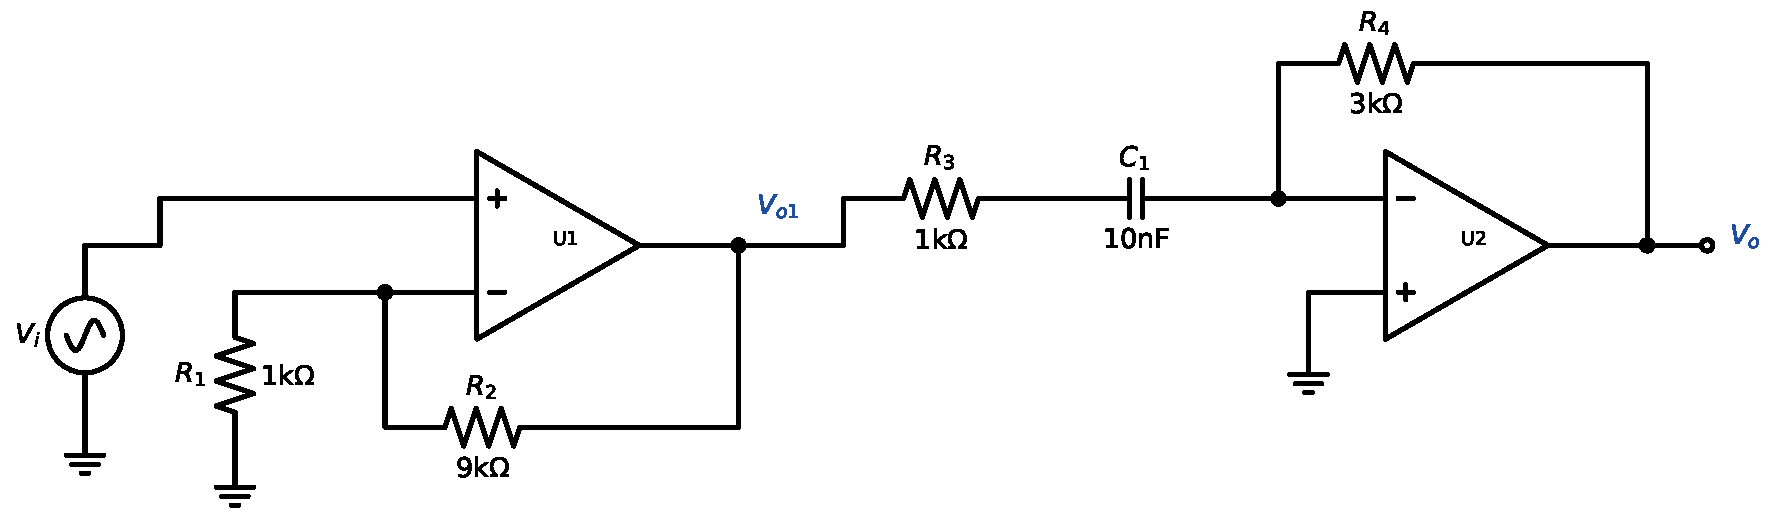
\includegraphics[width=\linewidth,height=5cm,keepaspectratio]{p08_circuit}\end{center}
\solstep{1}{What limits the input?}Every op-amp output must obey tool T6. For $V_i = A\sin(\omega_{in} t)$ each op-amp output is a sinusoid $|H_k(j\omega_{in})|A\sin(\omega_{in}t+\dots)$, so its fastest slope is $\omega_{in}|H_k(j\omega_{in})|A$. We need $|H_k(j\omega_{in})|$ from $V_i$ to each op-amp output ($V_{o1}$, $V_{o}$). Here $\omega_{in} = 2\pi\cdot3000 = 18800$\,rad/s and $SR = 0.5\,\mathrm{V}/\mu\mathrm{s} = 5\times 10^{5}\,\mathrm{V/s}$.
\solstep{2}{Gain to every op-amp output at $\omega_{in}$}Ideal op-amps: each block follows from its block formula (tool T2); a cascade multiplies, so $|H_k| = \prod_{j\le k}|\text{block } j|$.

\textbf{Block 1 (U1).} Non-inverting block: The $+$ input is the block input: $V_+ = V_{i}$. The op-amp forces $V_-=V_+$, and $R_{1}$, $R_{2}$ divide the output: $V_- = \frac{R_{1}}{R_{1} + R_{2}}V_{o1}$, hence $V_{o1} = \left(1+\frac{R_{2}}{R_{1}}\right)V_+$.\[
\frac{V_{o1}}{V_{i}} = \left(1+\frac{R_{2}}{R_{1}}\right) = 10
\]
At $s=j\omega_{in}$: $\left|\frac{V_{o1}}{V_{i}}\right| = 10$.

\textbf{Block 2 (U2).} Inverting block: the $+$ input is grounded, so $V_- = V_+ = 0$ (virtual ground). The current $\frac{V_{o1} - 0}{Z_{in2}}$ through $Z_{in2}$ cannot enter the op-amp, so all of it flows through $R_{4}$: $V_{o} = 0 - R_{4}\cdot\frac{V_{o1}}{Z_{in2}}$.\begin{align*}
Z_{in2} &= R_{3} + \frac{1}{sC_{1}} = \dfrac{1000\,s + 10^{8}}{s}
\end{align*}
\[
\frac{V_{o}}{V_{o1}} = -\frac{R_{4}}{Z_{in2}} = \dfrac{-3\,s}{s + 10^{5}}
\]
At $s=j\omega_{in}$: $\left|\frac{V_{o}}{V_{o1}}\right| = 0.5557$, so $|H_2| = 10\times0.5557 = 5.557$.

{\small (To evaluate a magnitude, put $s=j\omega_{in}$ and use $|a+jb|=\sqrt{a^2+b^2}$ for the numerator and the denominator separately.)}
\solstep{3}{Which output slews first?}\begin{center}\renewcommand{\arraystretch}{1.35}
\begin{tabular}{cccc}
\toprule
output & $|H_k(j\omega_{in})|$ & amplitude & max slope $\omega_{in}|H_k|A$ (V/s) \\
\midrule
$V_{o1}$ & $10$ & $10A$ & $1.885\times 10^{5}A$ \\
$V_{o}$ & $5.557$ & $5.557A$ & $1.047\times 10^{5}A$ \\
\bottomrule
\end{tabular}\end{center}
All op-amps have the same slew rate, so the output with the \emph{largest} gain, $V_{o1}$, reaches the limit first.
\solstep{4}{Maximum input amplitude}\[
\omega_{in}\,|H|\,A \le SR\ \Rightarrow\ A_{max} = \frac{SR}{\omega_{in}|H|} = \frac{5\times 10^{5}}{18800\times10} = 2.65\,\mathrm{V}
\]

\begin{ansbox}
$V_{o1}$ distorts first. $A_{max} = 2.65\,\mathrm{V}$ (input amplitude); at that point $V_{o1}$ has amplitude $26.5\,\mathrm{V}$.
\end{ansbox}

\newpage
\subsection*{Solution 2E.9 \hfill Medium}
\begin{center}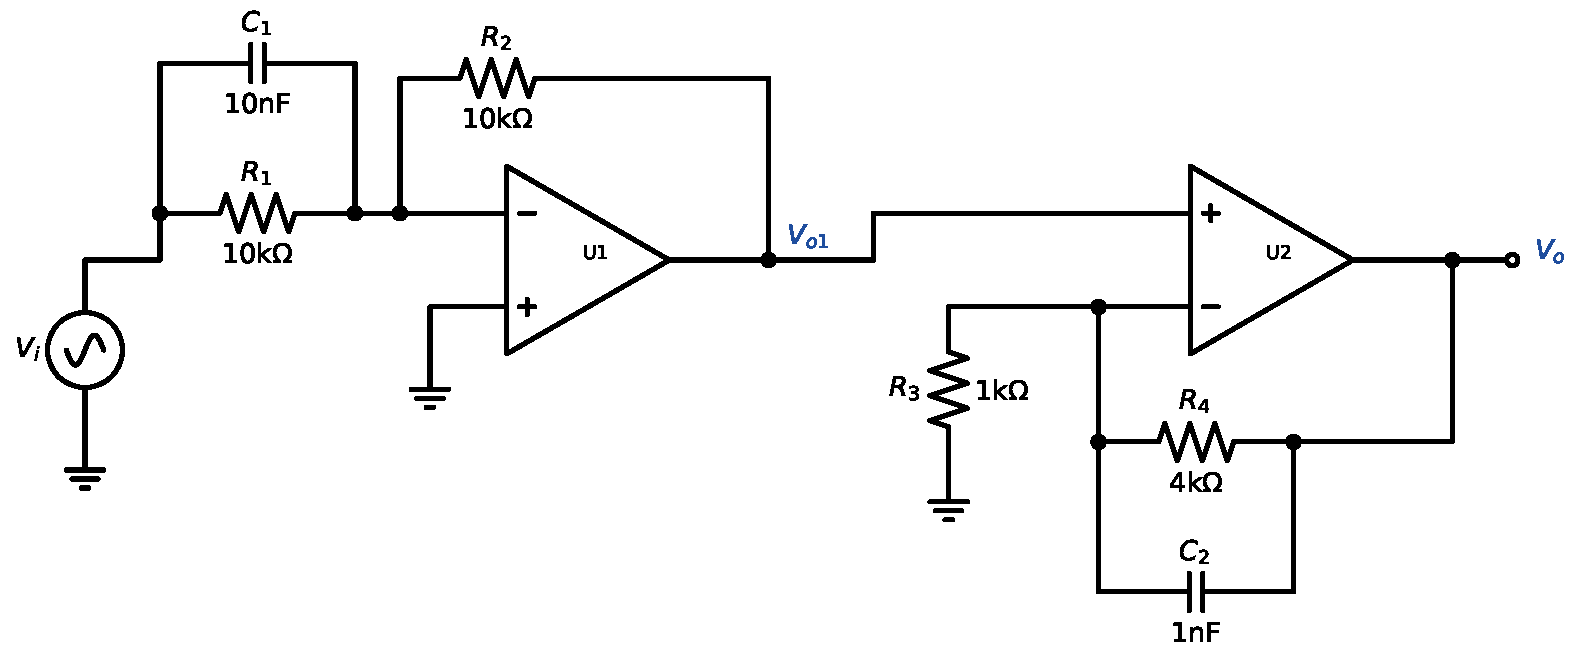
\includegraphics[width=\linewidth,height=5cm,keepaspectratio]{p09_circuit}\end{center}
\solstep{1}{What limits the input?}Every op-amp output must obey tool T6. For $V_i = A\sin(\omega_{in} t)$ each op-amp output is a sinusoid $|H_k(j\omega_{in})|A\sin(\omega_{in}t+\dots)$, so its fastest slope is $\omega_{in}|H_k(j\omega_{in})|A$. We need $|H_k(j\omega_{in})|$ from $V_i$ to each op-amp output ($V_{o1}$, $V_{o}$). Here $\omega_{in} = 2\pi\cdot10000 = 62800$\,rad/s and $SR = 1\,\mathrm{V}/\mu\mathrm{s} = 10^{6}\,\mathrm{V/s}$.
\solstep{2}{Gain to every op-amp output at $\omega_{in}$}Ideal op-amps: each block follows from its block formula (tool T2); a cascade multiplies, so $|H_k| = \prod_{j\le k}|\text{block } j|$.

\textbf{Block 1 (U1).} Inverting block: the $+$ input is grounded, so $V_- = V_+ = 0$ (virtual ground). The current $\frac{V_{i} - 0}{Z_{in1}}$ through $Z_{in1}$ cannot enter the op-amp, so all of it flows through $R_{2}$: $V_{o1} = 0 - R_{2}\cdot\frac{V_{i}}{Z_{in1}}$.\begin{align*}
Z_{in1} &= R_{1} \parallel \frac{1}{sC_{1}} = \dfrac{10^{8}}{s + 10000}
\end{align*}
\[
\frac{V_{o1}}{V_{i}} = -\frac{R_{2}}{Z_{in1}} = -10^{-4}\,s - 1
\]
At $s=j\omega_{in}$: $\left|\frac{V_{o1}}{V_{i}}\right| = 6.362$.

\textbf{Block 2 (U2).} Non-inverting block: The $+$ input is the block input: $V_+ = V_{o1}$. The op-amp forces $V_-=V_+$, and $R_{3}$, $Z_{f2}$ divide the output: $V_- = \frac{R_{3}}{R_{3} + Z_{f2}}V_{o}$, hence $V_{o} = \left(1+\frac{Z_{f2}}{R_{3}}\right)V_+$.\begin{align*}
Z_{f2} &= R_{4} \parallel \frac{1}{sC_{2}} = \dfrac{10^{9}}{s + 2.5\times 10^{5}}
\end{align*}
\[
\frac{V_{o}}{V_{o1}} = \left(1+\frac{Z_{f2}}{R_{3}}\right) = \dfrac{s + 1.25\times 10^{6}}{s + 2.5\times 10^{5}}
\]
At $s=j\omega_{in}$: $\left|\frac{V_{o}}{V_{o1}}\right| = 4.855$, so $|H_2| = 6.362\times4.855 = 30.89$.

{\small (To evaluate a magnitude, put $s=j\omega_{in}$ and use $|a+jb|=\sqrt{a^2+b^2}$ for the numerator and the denominator separately.)}
\solstep{3}{Which output slews first?}\begin{center}\renewcommand{\arraystretch}{1.35}
\begin{tabular}{cccc}
\toprule
output & $|H_k(j\omega_{in})|$ & amplitude & max slope $\omega_{in}|H_k|A$ (V/s) \\
\midrule
$V_{o1}$ & $6.362$ & $6.362A$ & $3.998\times 10^{5}A$ \\
$V_{o}$ & $30.89$ & $30.89A$ & $1.941\times 10^{6}A$ \\
\bottomrule
\end{tabular}\end{center}
All op-amps have the same slew rate, so the output with the \emph{largest} gain, $V_{o}$, reaches the limit first.
\solstep{4}{Maximum input amplitude}\[
\omega_{in}\,|H|\,A \le SR\ \Rightarrow\ A_{max} = \frac{SR}{\omega_{in}|H|} = \frac{10^{6}}{62800\times30.89} = 515\,\mathrm{m}\mathrm{V}
\]

\begin{ansbox}
$V_{o}$ distorts first. $A_{max} = 515\,\mathrm{m}\mathrm{V}$ (input amplitude); at that point $V_{o}$ has amplitude $15.9\,\mathrm{V}$.
\end{ansbox}

\newpage
\subsection*{Solution 2E.10 \hfill Medium}
\begin{center}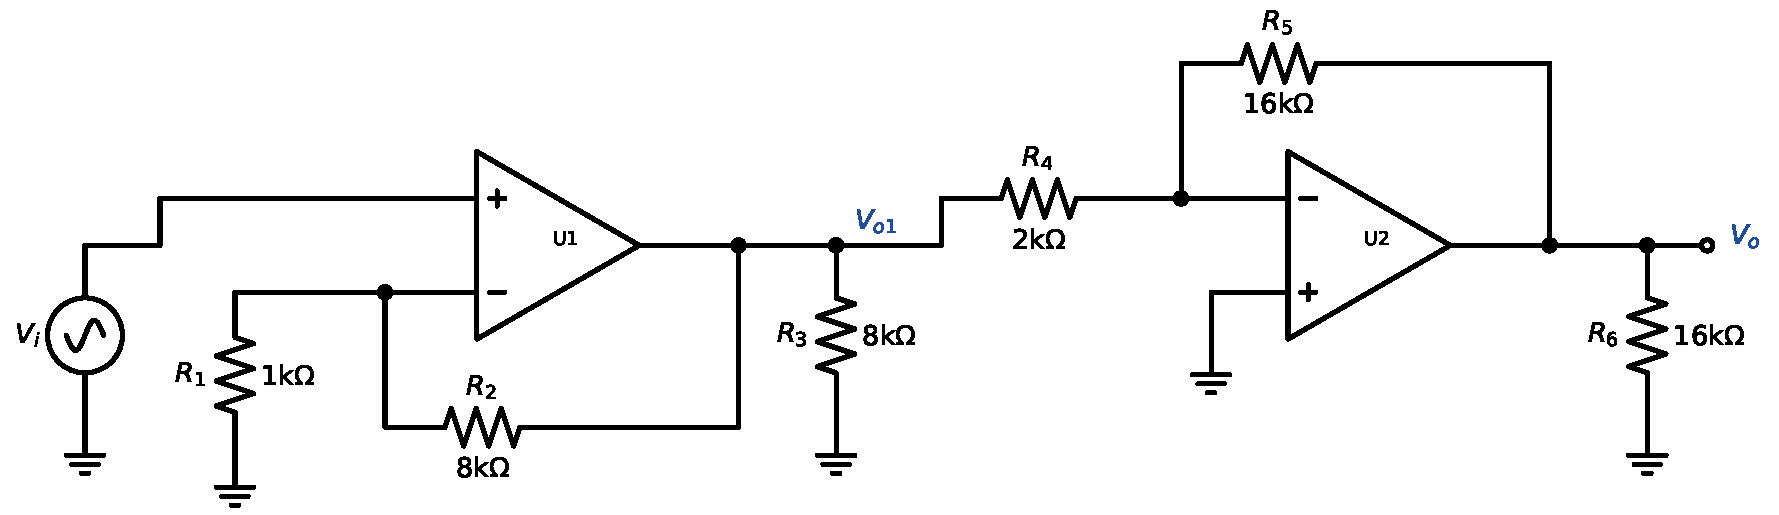
\includegraphics[width=\linewidth,height=5cm,keepaspectratio]{p10_circuit}\end{center}
\solstep{1}{What limits the input?}Every op-amp output must obey tool T6. For $V_i = A\sin(\omega_{in} t)$ each op-amp output is a sinusoid $|H_k(j\omega_{in})|A\sin(\omega_{in}t+\dots)$, so its fastest slope is $\omega_{in}|H_k(j\omega_{in})|A$. We need $|H_k(j\omega_{in})|$ from $V_i$ to each op-amp output ($V_{o1}$, $V_{o}$). Here $\omega_{in} = 2\pi\cdot2\times 10^{5} = 1.26\times 10^{6}$\,rad/s and $SR = 2\,\mathrm{V}/\mu\mathrm{s} = 2\times 10^{6}\,\mathrm{V/s}$.
\solstep{2}{Gain to every op-amp output at $\omega_{in}$}Each op-amp has $A(s)=\frac{10^{5}}{1+s/(2\pi\cdot20)}$, so each block is $\frac{A(\alpha_+-\alpha_-)}{1+A\beta}$ (tool T5; $\alpha,\beta$ from dividers, as in the finite-gain set).

\textbf{Block 1 (U1).} (no current enters either input, so both are plain dividers)\begin{align*}
V_+ &= V_{i} \\
V_- &= \frac{R_{1}}{R_{1}+R_{2}}V_{o1}
\end{align*}
\[
\frac{V_{o1}}{V_{i}} = \frac{A(\alpha_+-\alpha_-)}{1+A\beta} = \dfrac{1.26\times 10^{7}}{s + 1.4\times 10^{6}}
\]
At $s=j\omega_{in}$: $\left|\frac{V_{o1}}{V_{i}}\right| = 6.689$.

\textbf{Block 2 (U2).} (superposition: $V_{o1}$ alone with $V_{o}=0$ gives a divider $R_{4}$--$R_{5}$, and vice versa)\begin{align*}
V_+ &= 0 \quad(\text{grounded}) \\
V_- &= \frac{R_{5}}{R_{4}+R_{5}}V_{o1} + \frac{R_{4}}{R_{4}+R_{5}}V_{o}
\end{align*}
\[
\frac{V_{o}}{V_{o1}} = \frac{A(\alpha_+-\alpha_-)}{1+A\beta} = \dfrac{-1.12\times 10^{7}}{s + 1.4\times 10^{6}}
\]
At $s=j\omega_{in}$: $\left|\frac{V_{o}}{V_{o1}}\right| = 5.946$, so $|H_2| = 6.689\times5.946 = 39.78$.

{\small (To evaluate a magnitude, put $s=j\omega_{in}$ and use $|a+jb|=\sqrt{a^2+b^2}$ for the numerator and the denominator separately.)}
\solstep{3}{Which output slews first?}\begin{center}\renewcommand{\arraystretch}{1.35}
\begin{tabular}{cccc}
\toprule
output & $|H_k(j\omega_{in})|$ & amplitude & max slope $\omega_{in}|H_k|A$ (V/s) \\
\midrule
$V_{o1}$ & $6.689$ & $6.689A$ & $8.406\times 10^{6}A$ \\
$V_{o}$ & $39.78$ & $39.78A$ & $4.998\times 10^{7}A$ \\
\bottomrule
\end{tabular}\end{center}
All op-amps have the same slew rate, so the output with the \emph{largest} gain, $V_{o}$, reaches the limit first.
\solstep{4}{Maximum input amplitude}\[
\omega_{in}\,|H|\,A \le SR\ \Rightarrow\ A_{max} = \frac{SR}{\omega_{in}|H|} = \frac{2\times 10^{6}}{1.26\times 10^{6}\times39.78} = 40\,\mathrm{m}\mathrm{V}
\]

\begin{ansbox}
$V_{o}$ distorts first. $A_{max} = 40\,\mathrm{m}\mathrm{V}$ (input amplitude); at that point $V_{o}$ has amplitude $1.59\,\mathrm{V}$.
\end{ansbox}

\newpage
\subsection*{Solution 2E.11 \hfill Medium}
\begin{center}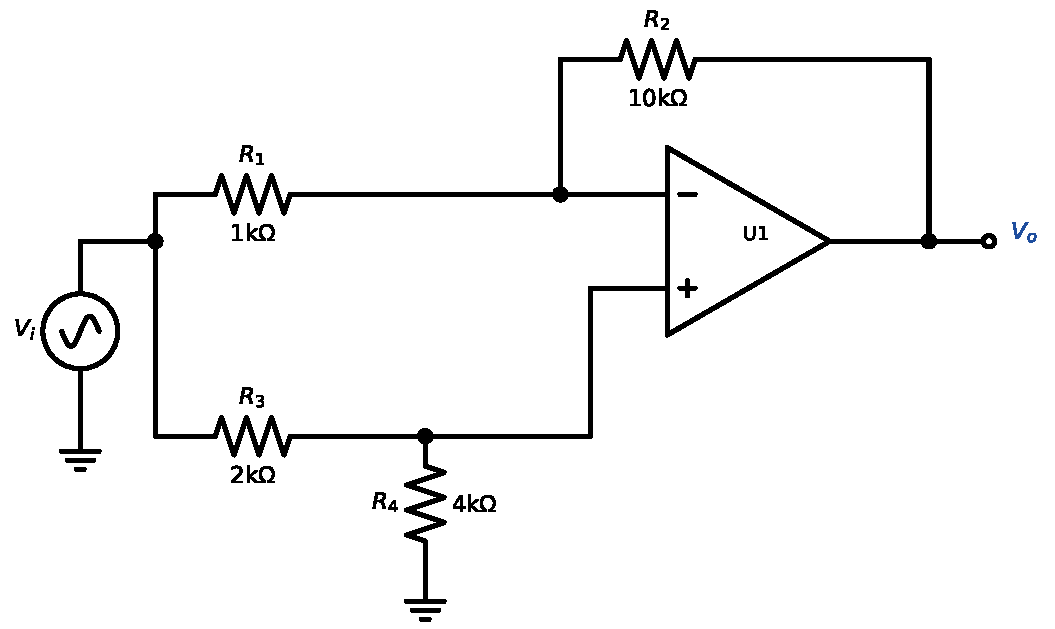
\includegraphics[width=\linewidth,height=5cm,keepaspectratio]{p11_circuit}\end{center}
\solstep{1}{What limits the input?}Every op-amp output must obey tool T6. For $V_i = A\sin(\omega_{in} t)$ each op-amp output is a sinusoid $|H_k(j\omega_{in})|A\sin(\omega_{in}t+\dots)$, so its fastest slope is $\omega_{in}|H_k(j\omega_{in})|A$. We need $|H_k(j\omega_{in})|$ from $V_i$ to the output. Here $\omega_{in} = 2\pi\cdot50000 = 3.14\times 10^{5}$\,rad/s and $SR = 3\,\mathrm{V}/\mu\mathrm{s} = 3\times 10^{6}\,\mathrm{V/s}$.
\solstep{2}{Gain to every op-amp output at $\omega_{in}$}Each op-amp has $A(s)=\frac{10^{5}}{1+s/(2\pi\cdot10)}$, so each block is $\frac{A(\alpha_+-\alpha_-)}{1+A\beta}$ (tool T5; $\alpha,\beta$ from dividers, as in the finite-gain set).

\textbf{Block 1 (U1).} (each input is a divider; the $-$ input sees both sources, use superposition)\begin{align*}
V_+ &= \frac{R_{4}}{R_{3}+R_{4}}V_{i} \\
V_- &= \frac{R_{2}}{R_{1}+R_{2}}V_{i} + \frac{R_{1}}{R_{1}+R_{2}}V_{o}
\end{align*}
\[
\frac{V_{o}}{V_{i}} = \frac{A(\alpha_+-\alpha_-)}{1+A\beta} = \dfrac{-1.52\times 10^{6}}{s + 5.71\times 10^{5}}
\]
At $s=j\omega_{in}$: $\left|\frac{V_{o}}{V_{i}}\right| = 2.336$.

{\small (To evaluate a magnitude, put $s=j\omega_{in}$ and use $|a+jb|=\sqrt{a^2+b^2}$ for the numerator and the denominator separately.)}
\solstep{3}{Which output slews first?}\begin{center}\renewcommand{\arraystretch}{1.35}
\begin{tabular}{cccc}
\toprule
output & $|H_k(j\omega_{in})|$ & amplitude & max slope $\omega_{in}|H_k|A$ (V/s) \\
\midrule
$V_{o}$ & $2.336$ & $2.336A$ & $7.34\times 10^{5}A$ \\
\bottomrule
\end{tabular}\end{center}
There is only one op-amp output.
\solstep{4}{Maximum input amplitude}\[
\omega_{in}\,|H|\,A \le SR\ \Rightarrow\ A_{max} = \frac{SR}{\omega_{in}|H|} = \frac{3\times 10^{6}}{3.14\times 10^{5}\times2.336} = 4.09\,\mathrm{V}
\]

\begin{ansbox}
$A_{max} = 4.09\,\mathrm{V}$ (input amplitude); at that point $V_{o}$ has amplitude $9.55\,\mathrm{V}$.
\end{ansbox}

\newpage
\subsection*{Solution 2E.12 \hfill Medium}
\begin{center}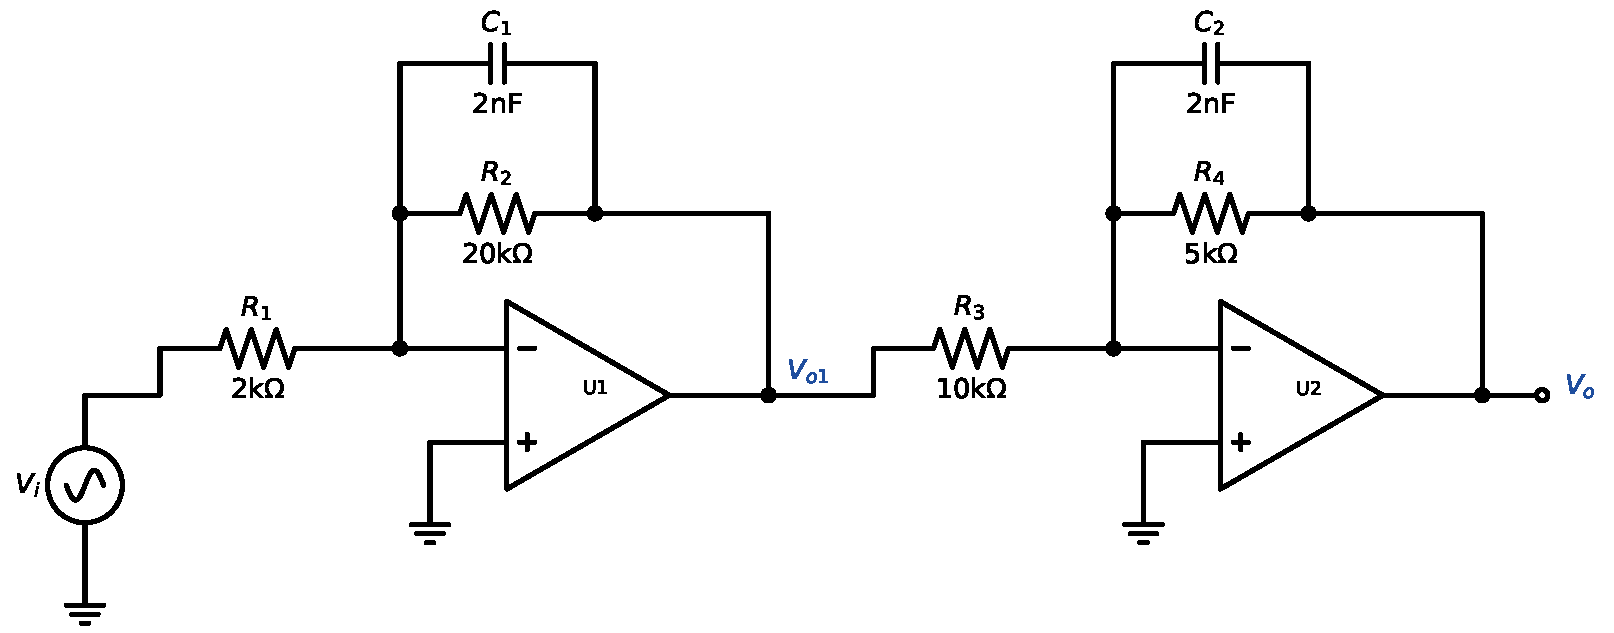
\includegraphics[width=\linewidth,height=5cm,keepaspectratio]{p12_circuit}\end{center}
\solstep{1}{What limits the input?}Every op-amp output must obey tool T6. For $V_i = A\sin(\omega_{in} t)$ each op-amp output is a sinusoid $|H_k(j\omega_{in})|A\sin(\omega_{in}t+\dots)$, so its fastest slope is $\omega_{in}|H_k(j\omega_{in})|A$. We need $|H_k(j\omega_{in})|$ from $V_i$ to each op-amp output ($V_{o1}$, $V_{o}$). Here $\omega_{in} = 2\pi\cdot8000 = 50300$\,rad/s and $SR = 0.5\,\mathrm{V}/\mu\mathrm{s} = 5\times 10^{5}\,\mathrm{V/s}$.
\solstep{2}{Gain to every op-amp output at $\omega_{in}$}Ideal op-amps: each block follows from its block formula (tool T2); a cascade multiplies, so $|H_k| = \prod_{j\le k}|\text{block } j|$.

\textbf{Block 1 (U1).} Inverting block: the $+$ input is grounded, so $V_- = V_+ = 0$ (virtual ground). The current $\frac{V_{i} - 0}{R_{1}}$ through $R_{1}$ cannot enter the op-amp, so all of it flows through $Z_{f1}$: $V_{o1} = 0 - Z_{f1}\cdot\frac{V_{i}}{R_{1}}$.\begin{align*}
Z_{f1} &= R_{2} \parallel \frac{1}{sC_{1}} = \dfrac{5\times 10^{8}}{s + 25000}
\end{align*}
\[
\frac{V_{o1}}{V_{i}} = -\frac{Z_{f1}}{R_{1}} = \dfrac{-2.5\times 10^{5}}{s + 25000}
\]
At $s=j\omega_{in}$: $\left|\frac{V_{o1}}{V_{i}}\right| = 4.453$.

\textbf{Block 2 (U2).} Inverting block: the $+$ input is grounded, so $V_- = V_+ = 0$ (virtual ground). The current $\frac{V_{o1} - 0}{R_{3}}$ through $R_{3}$ cannot enter the op-amp, so all of it flows through $Z_{f2}$: $V_{o} = 0 - Z_{f2}\cdot\frac{V_{o1}}{R_{3}}$.\begin{align*}
Z_{f2} &= R_{4} \parallel \frac{1}{sC_{2}} = \dfrac{5\times 10^{8}}{s + 10^{5}}
\end{align*}
\[
\frac{V_{o}}{V_{o1}} = -\frac{Z_{f2}}{R_{3}} = \dfrac{-50000}{s + 10^{5}}
\]
At $s=j\omega_{in}$: $\left|\frac{V_{o}}{V_{o1}}\right| = 0.4467$, so $|H_2| = 4.453\times0.4467 = 1.989$.

{\small (To evaluate a magnitude, put $s=j\omega_{in}$ and use $|a+jb|=\sqrt{a^2+b^2}$ for the numerator and the denominator separately.)}
\solstep{3}{Which output slews first?}\begin{center}\renewcommand{\arraystretch}{1.35}
\begin{tabular}{cccc}
\toprule
output & $|H_k(j\omega_{in})|$ & amplitude & max slope $\omega_{in}|H_k|A$ (V/s) \\
\midrule
$V_{o1}$ & $4.453$ & $4.453A$ & $2.238\times 10^{5}A$ \\
$V_{o}$ & $1.989$ & $1.989A$ & $100000A$ \\
\bottomrule
\end{tabular}\end{center}
All op-amps have the same slew rate, so the output with the \emph{largest} gain, $V_{o1}$, reaches the limit first.
\solstep{4}{Maximum input amplitude}\[
\omega_{in}\,|H|\,A \le SR\ \Rightarrow\ A_{max} = \frac{SR}{\omega_{in}|H|} = \frac{5\times 10^{5}}{50300\times4.453} = 2.23\,\mathrm{V}
\]

\begin{ansbox}
$V_{o1}$ distorts first. $A_{max} = 2.23\,\mathrm{V}$ (input amplitude); at that point $V_{o1}$ has amplitude $9.95\,\mathrm{V}$.
\end{ansbox}

\newpage
\subsection*{Solution 2E.13 \hfill Hard}
\begin{center}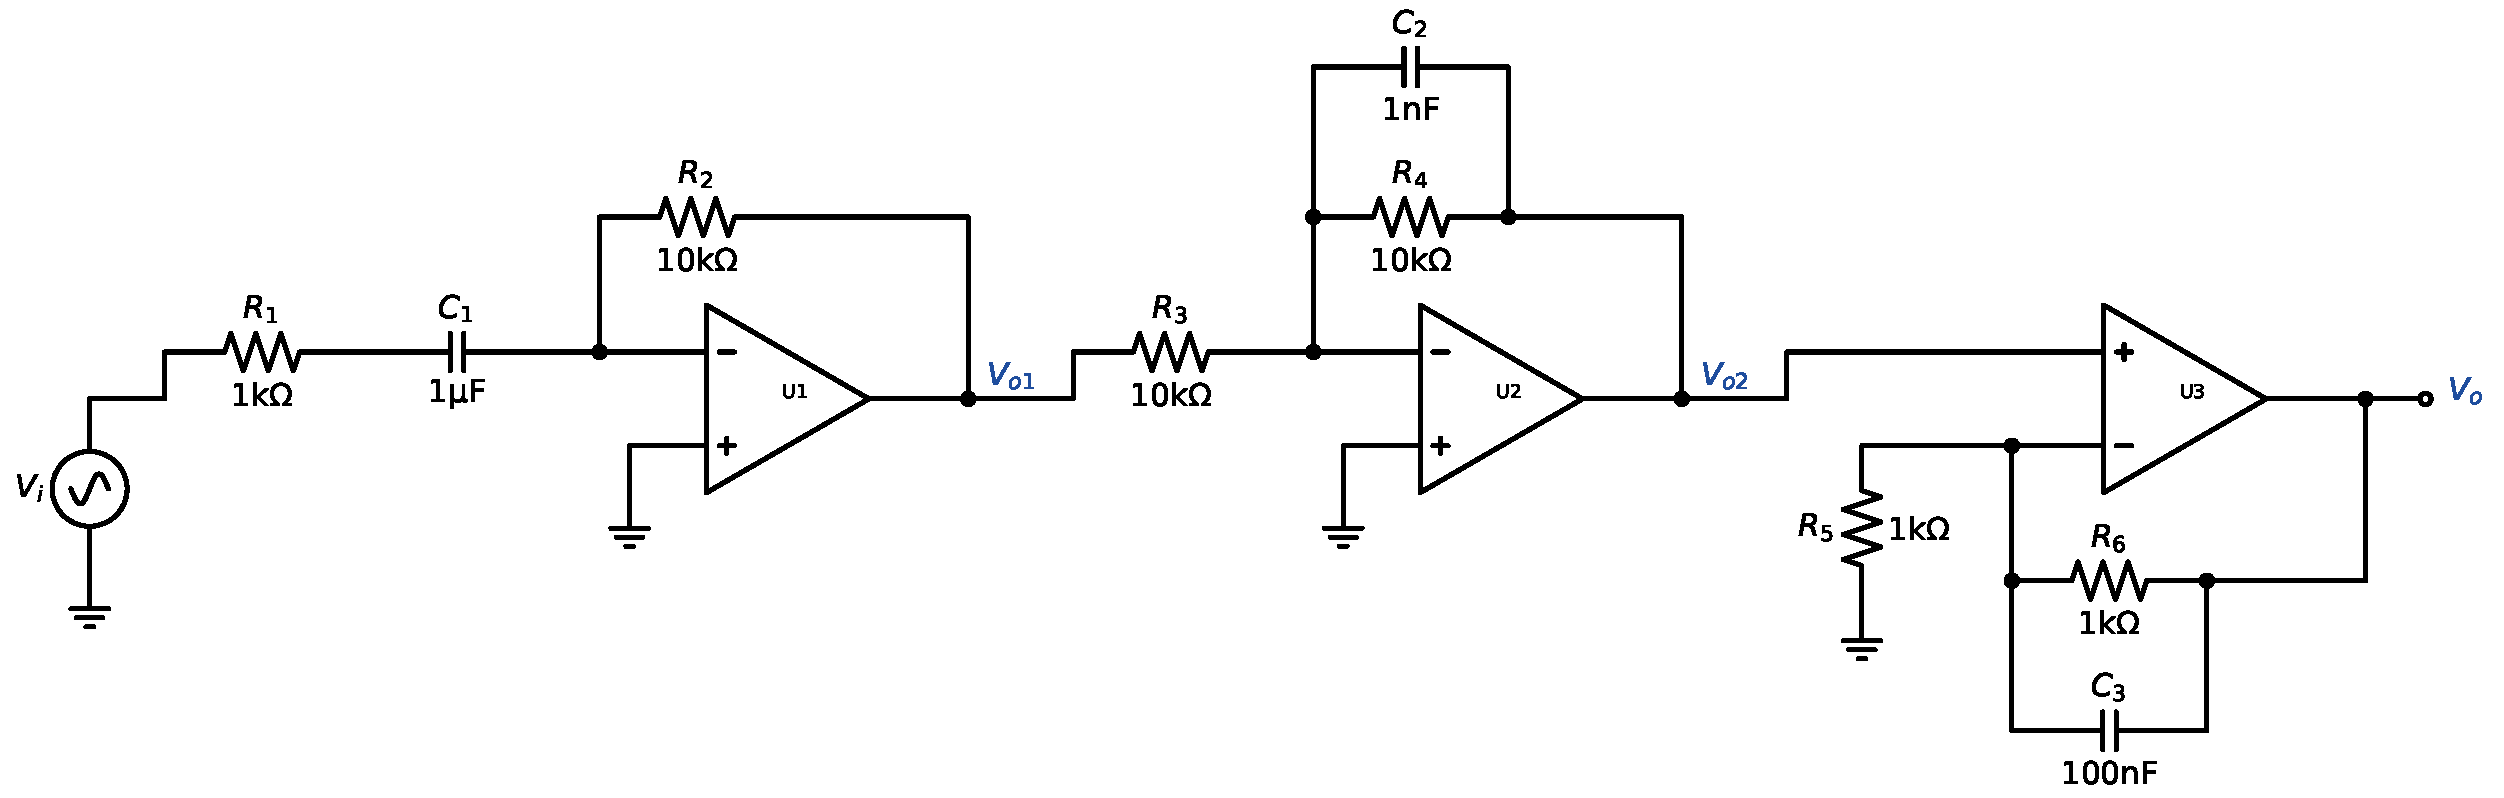
\includegraphics[width=\linewidth,height=5cm,keepaspectratio]{p13_circuit}\end{center}
\solstep{1}{What limits the input?}Every op-amp output must obey tool T6. For $V_i = A\sin(\omega_{in} t)$ each op-amp output is a sinusoid $|H_k(j\omega_{in})|A\sin(\omega_{in}t+\dots)$, so its fastest slope is $\omega_{in}|H_k(j\omega_{in})|A$. We need $|H_k(j\omega_{in})|$ from $V_i$ to each op-amp output ($V_{o1}$, $V_{o2}$, $V_{o}$). Here $\omega_{in} = 2\pi\cdot20000 = 1.26\times 10^{5}$\,rad/s and $SR = 1\,\mathrm{V}/\mu\mathrm{s} = 10^{6}\,\mathrm{V/s}$.
\solstep{2}{Gain to every op-amp output at $\omega_{in}$}Ideal op-amps: each block follows from its block formula (tool T2); a cascade multiplies, so $|H_k| = \prod_{j\le k}|\text{block } j|$.

\textbf{Block 1 (U1).} Inverting block: the $+$ input is grounded, so $V_- = V_+ = 0$ (virtual ground). The current $\frac{V_{i} - 0}{Z_{in1}}$ through $Z_{in1}$ cannot enter the op-amp, so all of it flows through $R_{2}$: $V_{o1} = 0 - R_{2}\cdot\frac{V_{i}}{Z_{in1}}$.\begin{align*}
Z_{in1} &= R_{1} + \frac{1}{sC_{1}} = \dfrac{1000\,s + 10^{6}}{s}
\end{align*}
\[
\frac{V_{o1}}{V_{i}} = -\frac{R_{2}}{Z_{in1}} = \dfrac{-10\,s}{s + 1000}
\]
At $s=j\omega_{in}$: $\left|\frac{V_{o1}}{V_{i}}\right| = 10$.

\textbf{Block 2 (U2).} Inverting block: the $+$ input is grounded, so $V_- = V_+ = 0$ (virtual ground). The current $\frac{V_{o1} - 0}{R_{3}}$ through $R_{3}$ cannot enter the op-amp, so all of it flows through $Z_{f2}$: $V_{o2} = 0 - Z_{f2}\cdot\frac{V_{o1}}{R_{3}}$.\begin{align*}
Z_{f2} &= R_{4} \parallel \frac{1}{sC_{2}} = \dfrac{10^{9}}{s + 10^{5}}
\end{align*}
\[
\frac{V_{o2}}{V_{o1}} = -\frac{Z_{f2}}{R_{3}} = \dfrac{-10^{5}}{s + 10^{5}}
\]
At $s=j\omega_{in}$: $\left|\frac{V_{o2}}{V_{o1}}\right| = 0.6227$, so $|H_2| = 10\times0.6227 = 6.227$.

\textbf{Block 3 (U3).} Non-inverting block: The $+$ input is the block input: $V_+ = V_{o2}$. The op-amp forces $V_-=V_+$, and $R_{5}$, $Z_{f3}$ divide the output: $V_- = \frac{R_{5}}{R_{5} + Z_{f3}}V_{o}$, hence $V_{o} = \left(1+\frac{Z_{f3}}{R_{5}}\right)V_+$.\begin{align*}
Z_{f3} &= R_{6} \parallel \frac{1}{sC_{3}} = \dfrac{10^{7}}{s + 10000}
\end{align*}
\[
\frac{V_{o}}{V_{o2}} = \left(1+\frac{Z_{f3}}{R_{5}}\right) = \dfrac{s + 20000}{s + 10000}
\]
At $s=j\omega_{in}$: $\left|\frac{V_{o}}{V_{o2}}\right| = 1.009$, so $|H_3| = 6.227\times1.009 = 6.285$.

{\small (To evaluate a magnitude, put $s=j\omega_{in}$ and use $|a+jb|=\sqrt{a^2+b^2}$ for the numerator and the denominator separately.)}
\solstep{3}{Which output slews first?}\begin{center}\renewcommand{\arraystretch}{1.35}
\begin{tabular}{cccc}
\toprule
output & $|H_k(j\omega_{in})|$ & amplitude & max slope $\omega_{in}|H_k|A$ (V/s) \\
\midrule
$V_{o1}$ & $10$ & $10A$ & $1.257\times 10^{6}A$ \\
$V_{o2}$ & $6.227$ & $6.227A$ & $7.825\times 10^{5}A$ \\
$V_{o}$ & $6.285$ & $6.285A$ & $7.898\times 10^{5}A$ \\
\bottomrule
\end{tabular}\end{center}
All op-amps have the same slew rate, so the output with the \emph{largest} gain, $V_{o1}$, reaches the limit first.
\solstep{4}{Maximum input amplitude}\[
\omega_{in}\,|H|\,A \le SR\ \Rightarrow\ A_{max} = \frac{SR}{\omega_{in}|H|} = \frac{10^{6}}{1.26\times 10^{5}\times10} = 796\,\mathrm{m}\mathrm{V}
\]

\begin{ansbox}
$V_{o1}$ distorts first. $A_{max} = 796\,\mathrm{m}\mathrm{V}$ (input amplitude); at that point $V_{o1}$ has amplitude $7.96\,\mathrm{V}$.
\end{ansbox}

\newpage
\subsection*{Solution 2E.14 \hfill Hard}
\begin{center}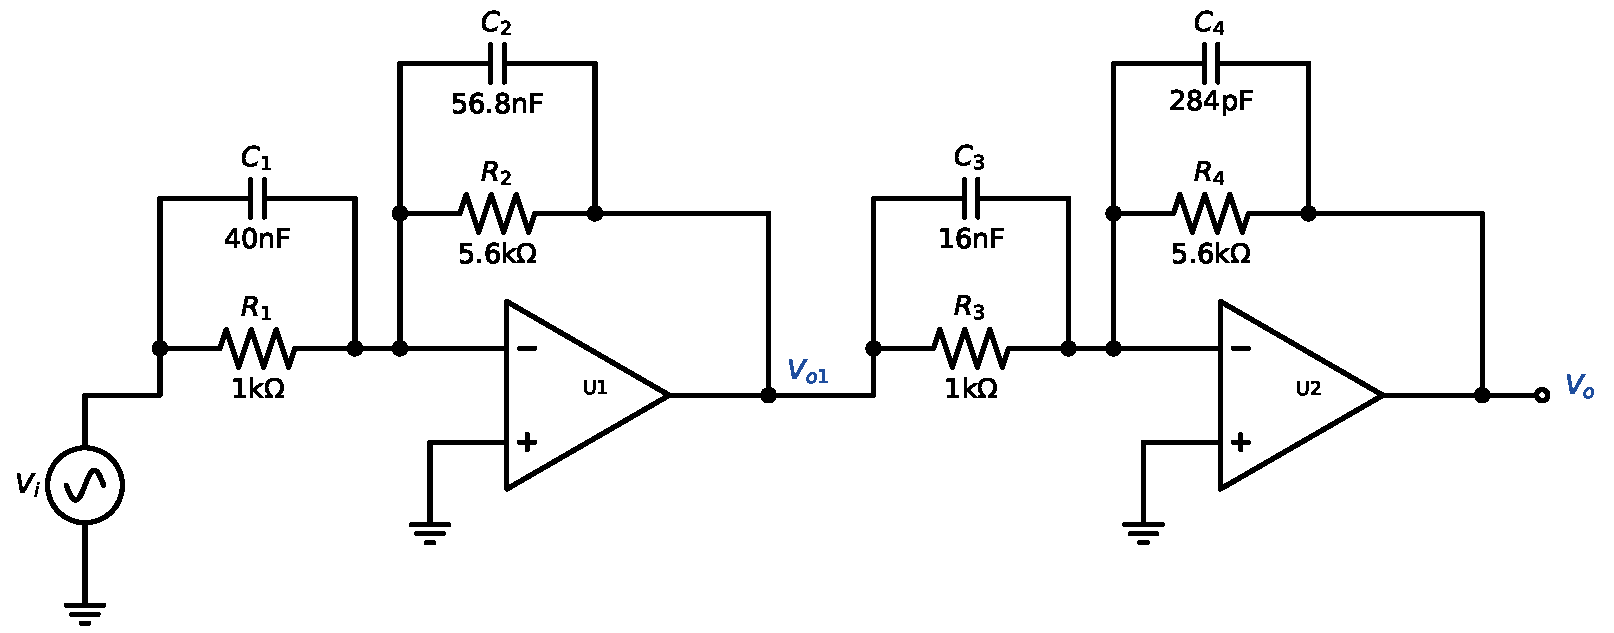
\includegraphics[width=\linewidth,height=5cm,keepaspectratio]{p14_circuit}\end{center}
\solstep{1}{What limits the input?}Every op-amp output must obey tool T6. For $V_i = A\sin(\omega_{in} t)$ each op-amp output is a sinusoid $|H_k(j\omega_{in})|A\sin(\omega_{in}t+\dots)$, so its fastest slope is $\omega_{in}|H_k(j\omega_{in})|A$. We need $|H_k(j\omega_{in})|$ from $V_i$ to each op-amp output ($V_{o1}$, $V_{o}$). Here $\omega_{in} = 2\pi\cdot2000 = 12600$\,rad/s and $SR = 0.5\,\mathrm{V}/\mu\mathrm{s} = 5\times 10^{5}\,\mathrm{V/s}$.
\solstep{2}{Gain to every op-amp output at $\omega_{in}$}Ideal op-amps: each block follows from its block formula (tool T2); a cascade multiplies, so $|H_k| = \prod_{j\le k}|\text{block } j|$.

\textbf{Block 1 (U1).} Inverting block: the $+$ input is grounded, so $V_- = V_+ = 0$ (virtual ground). The current $\frac{V_{i} - 0}{Z_{in1}}$ through $Z_{in1}$ cannot enter the op-amp, so all of it flows through $Z_{f1}$: $V_{o1} = 0 - Z_{f1}\cdot\frac{V_{i}}{Z_{in1}}$.\begin{align*}
Z_{in1} &= R_{1} \parallel \frac{1}{sC_{1}} = \dfrac{2.5\times 10^{7}}{s + 25000} \\
Z_{f1} &= R_{2} \parallel \frac{1}{sC_{2}} = \dfrac{1.76\times 10^{7}}{s + 3140}
\end{align*}
\[
\frac{V_{o1}}{V_{i}} = -\frac{Z_{f1}}{Z_{in1}} = \dfrac{-0.704\,s - 17600}{s + 3140}
\]
At $s=j\omega_{in}$: $\left|\frac{V_{o1}}{V_{i}}\right| = 1.521$.

\textbf{Block 2 (U2).} Inverting block: the $+$ input is grounded, so $V_- = V_+ = 0$ (virtual ground). The current $\frac{V_{o1} - 0}{Z_{in2}}$ through $Z_{in2}$ cannot enter the op-amp, so all of it flows through $Z_{f2}$: $V_{o} = 0 - Z_{f2}\cdot\frac{V_{o1}}{Z_{in2}}$.\begin{align*}
Z_{in2} &= R_{3} \parallel \frac{1}{sC_{3}} = \dfrac{6.25\times 10^{7}}{s + 62500} \\
Z_{f2} &= R_{4} \parallel \frac{1}{sC_{4}} = \dfrac{3.52\times 10^{9}}{s + 6.29\times 10^{5}}
\end{align*}
\[
\frac{V_{o}}{V_{o1}} = -\frac{Z_{f2}}{Z_{in2}} = \dfrac{-56.3\,s - 3.52\times 10^{6}}{s + 6.29\times 10^{5}}
\]
At $s=j\omega_{in}$: $\left|\frac{V_{o}}{V_{o1}}\right| = 5.711$, so $|H_2| = 1.521\times5.711 = 8.687$.

{\small (To evaluate a magnitude, put $s=j\omega_{in}$ and use $|a+jb|=\sqrt{a^2+b^2}$ for the numerator and the denominator separately.)}
\solstep{3}{Which output slews first?}\begin{center}\renewcommand{\arraystretch}{1.35}
\begin{tabular}{cccc}
\toprule
output & $|H_k(j\omega_{in})|$ & amplitude & max slope $\omega_{in}|H_k|A$ (V/s) \\
\midrule
$V_{o1}$ & $1.521$ & $1.521A$ & $19120A$ \\
$V_{o}$ & $8.687$ & $8.687A$ & $1.092\times 10^{5}A$ \\
\bottomrule
\end{tabular}\end{center}
All op-amps have the same slew rate, so the output with the \emph{largest} gain, $V_{o}$, reaches the limit first.
\solstep{4}{Maximum input amplitude}\[
\omega_{in}\,|H|\,A \le SR\ \Rightarrow\ A_{max} = \frac{SR}{\omega_{in}|H|} = \frac{5\times 10^{5}}{12600\times8.687} = 4.58\,\mathrm{V}
\]

\begin{ansbox}
$V_{o}$ distorts first. $A_{max} = 4.58\,\mathrm{V}$ (input amplitude); at that point $V_{o}$ has amplitude $39.8\,\mathrm{V}$.
\end{ansbox}

\newpage
\subsection*{Solution 2E.15 \hfill Hard}
\begin{center}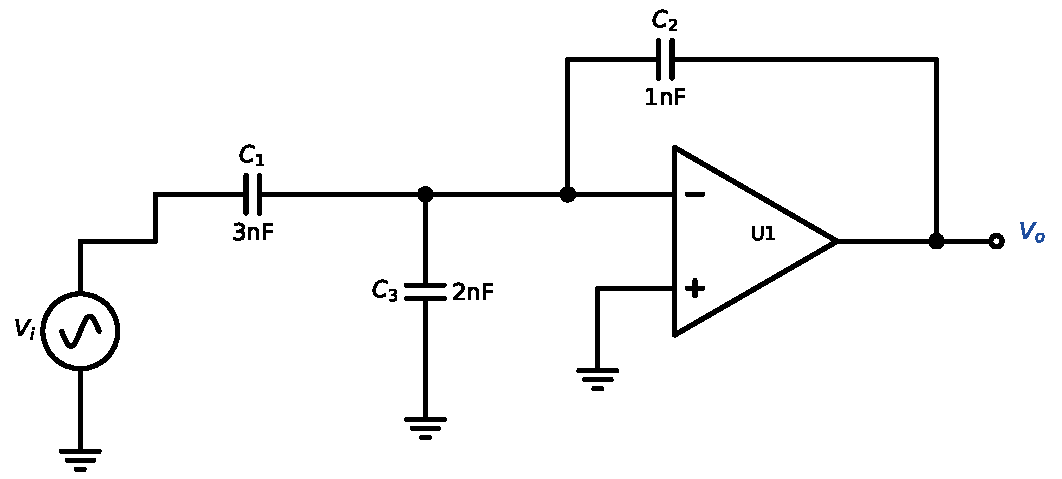
\includegraphics[width=\linewidth,height=5cm,keepaspectratio]{p15_circuit}\end{center}
\solstep{1}{What limits the input?}Every op-amp output must obey tool T6. For $V_i = A\sin(\omega_{in} t)$ each op-amp output is a sinusoid $|H_k(j\omega_{in})|A\sin(\omega_{in}t+\dots)$, so its fastest slope is $\omega_{in}|H_k(j\omega_{in})|A$. We need $|H_k(j\omega_{in})|$ from $V_i$ to the output. Here $\omega_{in} = 2\pi\cdot5\times 10^{5} = 3.14\times 10^{6}$\,rad/s and $SR = 5\,\mathrm{V}/\mu\mathrm{s} = 5\times 10^{6}\,\mathrm{V/s}$.
\solstep{2}{Gain to every op-amp output at $\omega_{in}$}Each op-amp has $A(s)=\frac{10^{5}}{1+s/(2\pi\cdot30)}$, so each block is $\frac{A(\alpha_+-\alpha_-)}{1+A\beta}$ (tool T5; $\alpha,\beta$ from dividers, as in the finite-gain set).

\textbf{Block 1 (U1).} (superposition: with $V_{o}=0$, $\frac{1}{sC_{2}}$ and $\frac{1}{sC_{3}}$ are in parallel from the $-$ input to ground; with $V_{i}=0$, $\frac{1}{sC_{1}}$ and $\frac{1}{sC_{3}}$ are. $\frac{1}{sC_{3}}$ matters now, because $V_-$ is no longer forced to 0.)\begin{align*}
V_+ &= 0 \quad(\text{grounded}) \\
V_- &= \frac{\frac{1}{sC_{2}}\parallel \frac{1}{sC_{3}}}{\frac{1}{sC_{1}}+\frac{1}{sC_{2}}\parallel \frac{1}{sC_{3}}}V_{i} + \frac{\frac{1}{sC_{1}}\parallel \frac{1}{sC_{3}}}{\frac{1}{sC_{2}}+\frac{1}{sC_{1}}\parallel \frac{1}{sC_{3}}}V_{o}
\end{align*}
\[
\frac{V_{o}}{V_{i}} = \frac{A(\alpha_+-\alpha_-)}{1+A\beta} = \dfrac{-9.42\times 10^{6}}{s + 3.14\times 10^{6}}
\]
At $s=j\omega_{in}$: $\left|\frac{V_{o}}{V_{i}}\right| = 2.121$.

{\small (To evaluate a magnitude, put $s=j\omega_{in}$ and use $|a+jb|=\sqrt{a^2+b^2}$ for the numerator and the denominator separately.)}
\solstep{3}{Which output slews first?}\begin{center}\renewcommand{\arraystretch}{1.35}
\begin{tabular}{cccc}
\toprule
output & $|H_k(j\omega_{in})|$ & amplitude & max slope $\omega_{in}|H_k|A$ (V/s) \\
\midrule
$V_{o}$ & $2.121$ & $2.121A$ & $6.664\times 10^{6}A$ \\
\bottomrule
\end{tabular}\end{center}
There is only one op-amp output.
\solstep{4}{Maximum input amplitude}\[
\omega_{in}\,|H|\,A \le SR\ \Rightarrow\ A_{max} = \frac{SR}{\omega_{in}|H|} = \frac{5\times 10^{6}}{3.14\times 10^{6}\times2.121} = 750\,\mathrm{m}\mathrm{V}
\]

\begin{ansbox}
$A_{max} = 750\,\mathrm{m}\mathrm{V}$ (input amplitude); at that point $V_{o}$ has amplitude $1.59\,\mathrm{V}$.
\end{ansbox}

\newpage
\subsection*{Solution 2E.16 \hfill Hard}
\begin{center}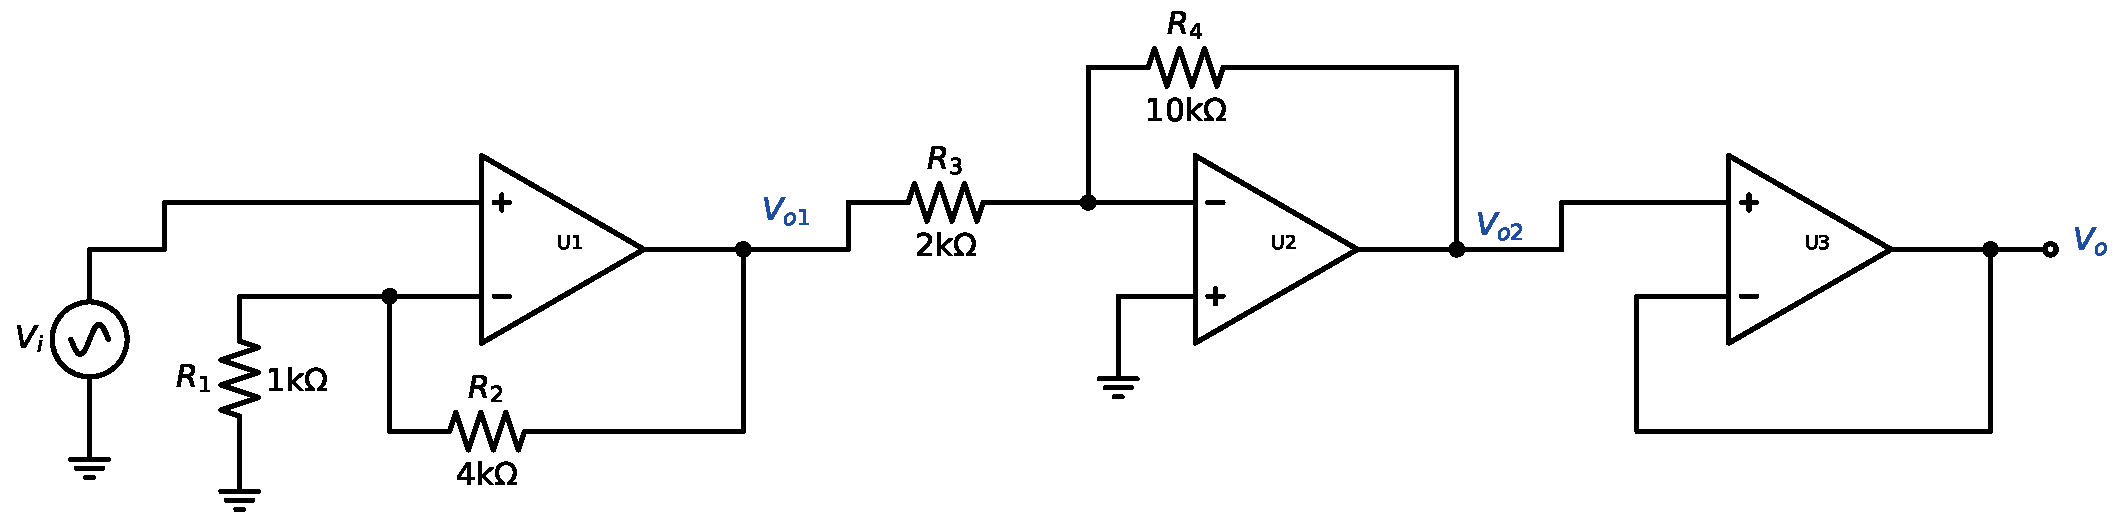
\includegraphics[width=\linewidth,height=5cm,keepaspectratio]{p16_circuit}\end{center}
\solstep{1}{What limits the input?}Every op-amp output must obey tool T6. For $V_i = A\sin(\omega_{in} t)$ each op-amp output is a sinusoid $|H_k(j\omega_{in})|A\sin(\omega_{in}t+\dots)$, so its fastest slope is $\omega_{in}|H_k(j\omega_{in})|A$. We need $|H_k(j\omega_{in})|$ from $V_i$ to each op-amp output ($V_{o1}$, $V_{o2}$, $V_{o}$). Here $\omega_{in} = 2\pi\cdot10^{5} = 6.28\times 10^{5}$\,rad/s and $SR = 2\,\mathrm{V}/\mu\mathrm{s} = 2\times 10^{6}\,\mathrm{V/s}$.
\solstep{2}{Gain to every op-amp output at $\omega_{in}$}Each op-amp has $A(s)=\frac{10^{5}}{1+s/(2\pi\cdot10)}$, so each block is $\frac{A(\alpha_+-\alpha_-)}{1+A\beta}$ (tool T5; $\alpha,\beta$ from dividers, as in the finite-gain set).

\textbf{Block 1 (U1).} (no current enters either input, so both are plain dividers)\begin{align*}
V_+ &= V_{i} \\
V_- &= \frac{R_{1}}{R_{1}+R_{2}}V_{o1}
\end{align*}
\[
\frac{V_{o1}}{V_{i}} = \frac{A(\alpha_+-\alpha_-)}{1+A\beta} = \dfrac{6.28\times 10^{6}}{s + 1.26\times 10^{6}}
\]
At $s=j\omega_{in}$: $\left|\frac{V_{o1}}{V_{i}}\right| = 4.472$.

\textbf{Block 2 (U2).} (superposition: $V_{o1}$ alone with $V_{o2}=0$ gives a divider $R_{3}$--$R_{4}$, and vice versa)\begin{align*}
V_+ &= 0 \quad(\text{grounded}) \\
V_- &= \frac{R_{4}}{R_{3}+R_{4}}V_{o1} + \frac{R_{3}}{R_{3}+R_{4}}V_{o2}
\end{align*}
\[
\frac{V_{o2}}{V_{o1}} = \frac{A(\alpha_+-\alpha_-)}{1+A\beta} = \dfrac{-5.24\times 10^{6}}{s + 1.05\times 10^{6}}
\]
At $s=j\omega_{in}$: $\left|\frac{V_{o2}}{V_{o1}}\right| = 4.287$, so $|H_2| = 4.472\times4.287 = 19.17$.

\textbf{Block 3 (U3).} (no current enters either input, so both are plain dividers)\begin{align*}
V_+ &= V_{o2} \\
V_- &= V_{o}
\end{align*}
\[
\frac{V_{o}}{V_{o2}} = \frac{A(\alpha_+-\alpha_-)}{1+A\beta} = \dfrac{6.28\times 10^{6}}{s + 6.28\times 10^{6}}
\]
At $s=j\omega_{in}$: $\left|\frac{V_{o}}{V_{o2}}\right| = 0.995$, so $|H_3| = 19.17\times0.995 = 19.08$.

{\small (To evaluate a magnitude, put $s=j\omega_{in}$ and use $|a+jb|=\sqrt{a^2+b^2}$ for the numerator and the denominator separately.)}
\solstep{3}{Which output slews first?}\begin{center}\renewcommand{\arraystretch}{1.35}
\begin{tabular}{cccc}
\toprule
output & $|H_k(j\omega_{in})|$ & amplitude & max slope $\omega_{in}|H_k|A$ (V/s) \\
\midrule
$V_{o1}$ & $4.472$ & $4.472A$ & $2.81\times 10^{6}A$ \\
$V_{o2}$ & $19.17$ & $19.17A$ & $1.205\times 10^{7}A$ \\
$V_{o}$ & $19.08$ & $19.08A$ & $1.199\times 10^{7}A$ \\
\bottomrule
\end{tabular}\end{center}
All op-amps have the same slew rate, so the output with the \emph{largest} gain, $V_{o2}$, reaches the limit first.
\solstep{4}{Maximum input amplitude}\[
\omega_{in}\,|H|\,A \le SR\ \Rightarrow\ A_{max} = \frac{SR}{\omega_{in}|H|} = \frac{2\times 10^{6}}{6.28\times 10^{5}\times19.17} = 166\,\mathrm{m}\mathrm{V}
\]

\begin{ansbox}
$V_{o2}$ distorts first. $A_{max} = 166\,\mathrm{m}\mathrm{V}$ (input amplitude); at that point $V_{o2}$ has amplitude $3.18\,\mathrm{V}$.
\end{ansbox}

\newpage
\subsection*{Solution 2E.17 \hfill Hard}
\begin{center}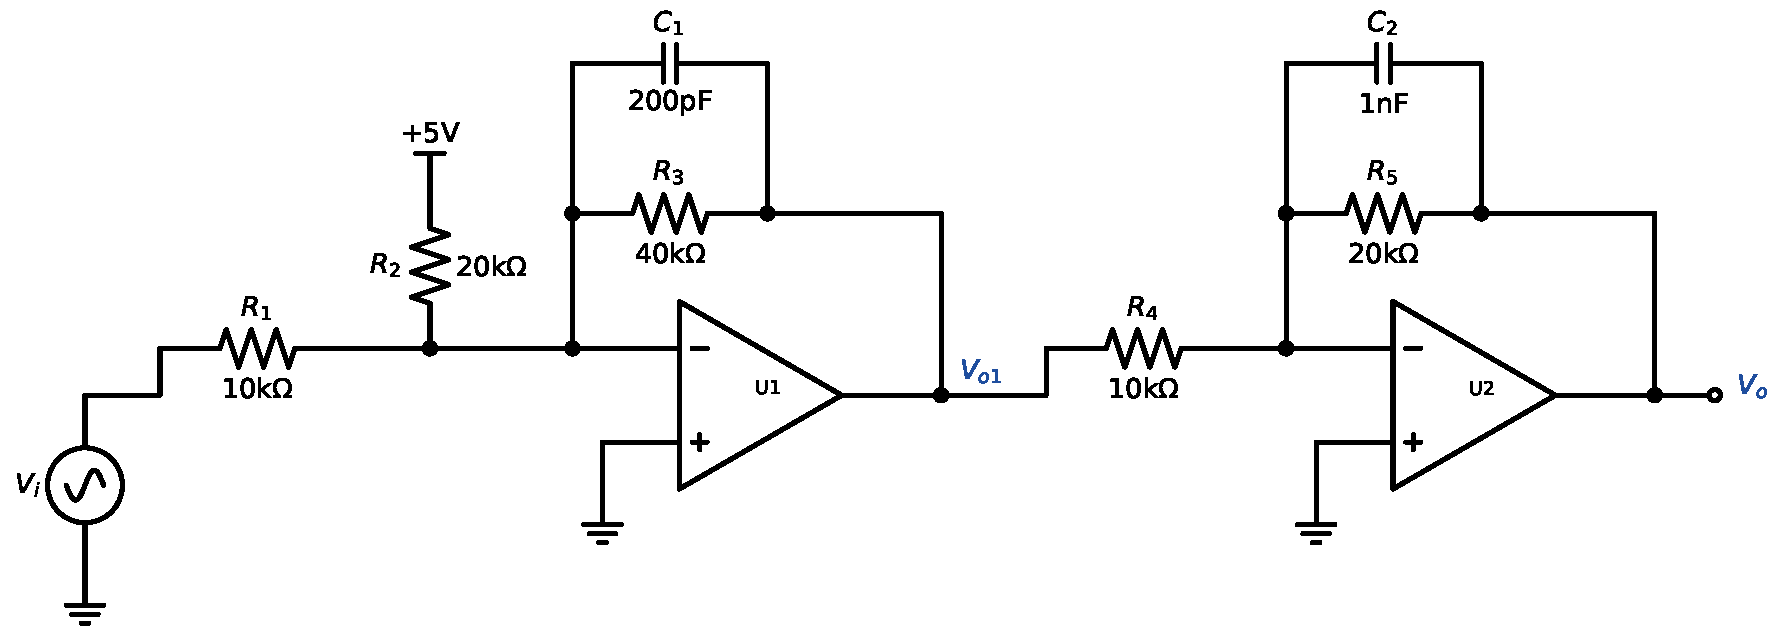
\includegraphics[width=\linewidth,height=5cm,keepaspectratio]{p17_circuit}\end{center}
\solstep{1}{What limits the input?}Every op-amp output must obey tool T6. For $V_i = A\sin(\omega_{in} t)$ each op-amp output is a sinusoid $|H_k(j\omega_{in})|A\sin(\omega_{in}t+\dots)$, so its fastest slope is $\omega_{in}|H_k(j\omega_{in})|A$. We need $|H_k(j\omega_{in})|$ from $V_i$ to each op-amp output ($V_{o1}$, $V_{o}$). Here $\omega_{in} = 2\pi\cdot10000 = 62800$\,rad/s and $SR = 0.2\,\mathrm{V}/\mu\mathrm{s} = 2\times 10^{5}\,\mathrm{V/s}$. (A DC offset does not change the slope of a signal, so only the AC part matters.)
\solstep{2}{Gain to every op-amp output at $\omega_{in}$}Ideal op-amps: each block follows from its block formula (tool T2); a cascade multiplies, so $|H_k| = \prod_{j\le k}|\text{block } j|$.

\textbf{Block 1 (U1).} Summing block: $V_-=V_+=0$ (virtual ground), so the input currents $\frac{V_{i}}{R_{1}}$ and $\frac{V_{DC}}{R_{2}}$ simply add and both flow through $Z_{f1}$: $V_{o1} = -Z_{f1}\left(\frac{V_{i}}{R_{1}} + \frac{V_{DC}}{R_{2}}\right)$. For the AC part the supply is zero, so $R_{2}$ (from virtual ground to AC ground) carries no AC current and drops out.\begin{align*}
Z_{f1} &= R_{3} \parallel \frac{1}{sC_{1}} = \dfrac{5\times 10^{9}}{s + 1.25\times 10^{5}}
\end{align*}
\[
\frac{V_{o1}}{V_{i}} = -\frac{Z_{f1}}{R_{1}} = \dfrac{-5\times 10^{5}}{s + 1.25\times 10^{5}}
\]
At $s=j\omega_{in}$: $\left|\frac{V_{o1}}{V_{i}}\right| = 3.574$.

\textbf{Block 2 (U2).} Inverting block: the $+$ input is grounded, so $V_- = V_+ = 0$ (virtual ground). The current $\frac{V_{o1} - 0}{R_{4}}$ through $R_{4}$ cannot enter the op-amp, so all of it flows through $Z_{f2}$: $V_{o} = 0 - Z_{f2}\cdot\frac{V_{o1}}{R_{4}}$.\begin{align*}
Z_{f2} &= R_{5} \parallel \frac{1}{sC_{2}} = \dfrac{10^{9}}{s + 50000}
\end{align*}
\[
\frac{V_{o}}{V_{o1}} = -\frac{Z_{f2}}{R_{4}} = \dfrac{-10^{5}}{s + 50000}
\]
At $s=j\omega_{in}$: $\left|\frac{V_{o}}{V_{o1}}\right| = 1.245$, so $|H_2| = 3.574\times1.245 = 4.451$.

{\small (To evaluate a magnitude, put $s=j\omega_{in}$ and use $|a+jb|=\sqrt{a^2+b^2}$ for the numerator and the denominator separately.)}
\solstep{3}{Which output slews first?}\begin{center}\renewcommand{\arraystretch}{1.35}
\begin{tabular}{cccc}
\toprule
output & $|H_k(j\omega_{in})|$ & amplitude & max slope $\omega_{in}|H_k|A$ (V/s) \\
\midrule
$V_{o1}$ & $3.574$ & $3.574A$ & $2.246\times 10^{5}A$ \\
$V_{o}$ & $4.451$ & $4.451A$ & $2.797\times 10^{5}A$ \\
\bottomrule
\end{tabular}\end{center}
All op-amps have the same slew rate, so the output with the \emph{largest} gain, $V_{o}$, reaches the limit first.
\solstep{4}{Maximum input amplitude}\[
\omega_{in}\,|H|\,A \le SR\ \Rightarrow\ A_{max} = \frac{SR}{\omega_{in}|H|} = \frac{2\times 10^{5}}{62800\times4.451} = 715\,\mathrm{m}\mathrm{V}
\]

\begin{ansbox}
$V_{o}$ distorts first. $A_{max} = 715\,\mathrm{m}\mathrm{V}$ (input amplitude); at that point $V_{o}$ has amplitude $3.18\,\mathrm{V}$.
\end{ansbox}

\newpage
\subsection*{Solution 2E.18 \hfill Hard}
\begin{center}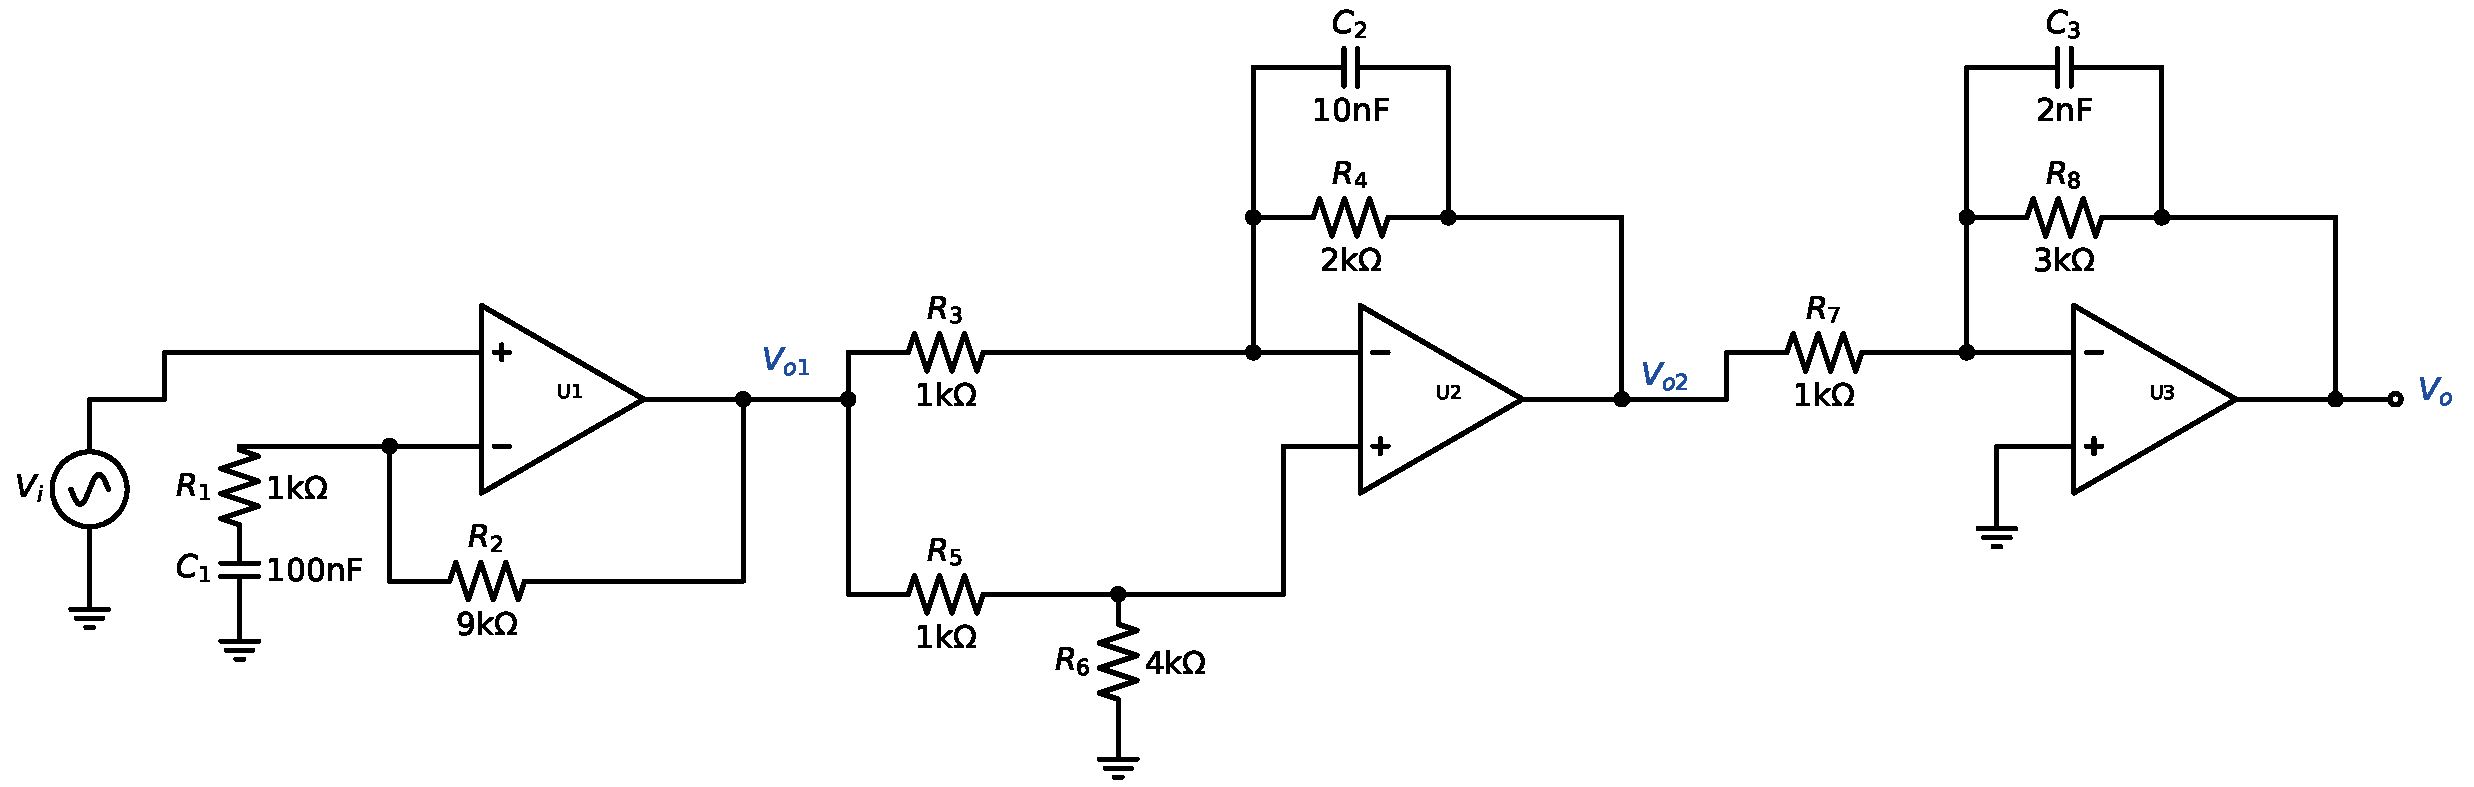
\includegraphics[width=\linewidth,height=5cm,keepaspectratio]{p18_circuit}\end{center}
\solstep{1}{What limits the input?}Every op-amp output must obey tool T6. For $V_i = A\sin(\omega_{in} t)$ each op-amp output is a sinusoid $|H_k(j\omega_{in})|A\sin(\omega_{in}t+\dots)$, so its fastest slope is $\omega_{in}|H_k(j\omega_{in})|A$. We need $|H_k(j\omega_{in})|$ from $V_i$ to each op-amp output ($V_{o1}$, $V_{o2}$, $V_{o}$). Here $\omega_{in} = 2\pi\cdot6000 = 37700$\,rad/s and $SR = 0.8\,\mathrm{V}/\mu\mathrm{s} = 8\times 10^{5}\,\mathrm{V/s}$.
\solstep{2}{Gain to every op-amp output at $\omega_{in}$}Ideal op-amps: each block follows from its block formula (tool T2); a cascade multiplies, so $|H_k| = \prod_{j\le k}|\text{block } j|$.

\textbf{Block 1 (U1).} Non-inverting block: The $+$ input is the block input: $V_+ = V_{i}$. The op-amp forces $V_-=V_+$, and $Z_{g1}$, $R_{2}$ divide the output: $V_- = \frac{Z_{g1}}{Z_{g1} + R_{2}}V_{o1}$, hence $V_{o1} = \left(1+\frac{R_{2}}{Z_{g1}}\right)V_+$.\begin{align*}
Z_{g1} &= R_{1} + \frac{1}{sC_{1}} = \dfrac{1000\,s + 10^{7}}{s}
\end{align*}
\[
\frac{V_{o1}}{V_{i}} = \left(1+\frac{R_{2}}{Z_{g1}}\right) = \dfrac{10\,s + 10000}{s + 10000}
\]
At $s=j\omega_{in}$: $\left|\frac{V_{o1}}{V_{i}}\right| = 9.669$.

\textbf{Block 2 (U2).} Difference block (both inputs driven by $V_{o1}$): use superposition. Through the $+$ path the signal is divided, $V_+ = \frac{R_{6}}{R_{5}+R_{6}}V_{o1}$, and amplified by the non-inverting gain $1+\frac{Z_{f2}}{R_{3}}$; through the $-$ path it is amplified by the inverting gain $-\frac{Z_{f2}}{R_{3}}$. Add the two contributions.\begin{align*}
Z_{f2} &= R_{4} \parallel \frac{1}{sC_{2}} = \dfrac{10^{8}}{s + 50000}
\end{align*}
\[
\frac{V_{o2}}{V_{o1}} = \frac{R_{6}}{R_{5}+R_{6}}\left(1+\frac{Z_{f2}}{R_{3}}\right) - \frac{Z_{f2}}{R_{3}} = \dfrac{0.8\,s + 20000}{s + 50000}
\]
At $s=j\omega_{in}$: $\left|\frac{V_{o2}}{V_{o1}}\right| = 0.5779$, so $|H_2| = 9.669\times0.5779 = 5.588$.

\textbf{Block 3 (U3).} Inverting block: the $+$ input is grounded, so $V_- = V_+ = 0$ (virtual ground). The current $\frac{V_{o2} - 0}{R_{7}}$ through $R_{7}$ cannot enter the op-amp, so all of it flows through $Z_{f3}$: $V_{o} = 0 - Z_{f3}\cdot\frac{V_{o2}}{R_{7}}$.\begin{align*}
Z_{f3} &= R_{8} \parallel \frac{1}{sC_{3}} = \dfrac{5\times 10^{8}}{s + 1.67\times 10^{5}}
\end{align*}
\[
\frac{V_{o}}{V_{o2}} = -\frac{Z_{f3}}{R_{7}} = \dfrac{-5\times 10^{5}}{s + 1.67\times 10^{5}}
\]
At $s=j\omega_{in}$: $\left|\frac{V_{o}}{V_{o2}}\right| = 2.926$, so $|H_3| = 5.588\times2.926 = 16.35$.

{\small (To evaluate a magnitude, put $s=j\omega_{in}$ and use $|a+jb|=\sqrt{a^2+b^2}$ for the numerator and the denominator separately.)}
\solstep{3}{Which output slews first?}\begin{center}\renewcommand{\arraystretch}{1.35}
\begin{tabular}{cccc}
\toprule
output & $|H_k(j\omega_{in})|$ & amplitude & max slope $\omega_{in}|H_k|A$ (V/s) \\
\midrule
$V_{o1}$ & $9.669$ & $9.669A$ & $3.645\times 10^{5}A$ \\
$V_{o2}$ & $5.588$ & $5.588A$ & $2.107\times 10^{5}A$ \\
$V_{o}$ & $16.35$ & $16.35A$ & $6.164\times 10^{5}A$ \\
\bottomrule
\end{tabular}\end{center}
All op-amps have the same slew rate, so the output with the \emph{largest} gain, $V_{o}$, reaches the limit first.
\solstep{4}{Maximum input amplitude}\[
\omega_{in}\,|H|\,A \le SR\ \Rightarrow\ A_{max} = \frac{SR}{\omega_{in}|H|} = \frac{8\times 10^{5}}{37700\times16.35} = 1.3\,\mathrm{V}
\]

\begin{ansbox}
$V_{o}$ distorts first. $A_{max} = 1.3\,\mathrm{V}$ (input amplitude); at that point $V_{o}$ has amplitude $21.2\,\mathrm{V}$.
\end{ansbox}

\end{document}
